%%%%%%%%%%%%%%%%%%%%%%%%%%%%%%%%%%%%%%%%%%%%%%%%%%%%%%%%%%%%%%%%%%%%%%%%%%%%%%%%%%%%%%%%%%%%%%%%%%%%%
% This template is distributed with ABSOLUTELY NO WARRANTY.
% It serves as a guideline and constitutes a basic structure for a
% thesis/dissertation. The user assumes full responsibility for formatting
% and typesetting their document and for verifying that all the thesis
% requirements set by the University of Tennessee are met. Please refer to the most
% recent UT thesis guide (http://web.utk.edu/~thesis/thesisresources.shtml)
% or contact the thesis consultant (http://web.utk.edu/~thesis/).
% Please report any bugs to the thesis consultant.
%%%%%%%%%%%%%%%%%%%%%%%%%%%%%%%%%%%%%%%%%%%%%%%%%%%%%%%%%%%%%%%%%%%%%%%%%%%%%%%%%%%%%%%%%%%%%%%%%%%%%
% O P T I O N S:
% 1. thesis/dissertation
% 2. monochrome
% 3. all options provided by the report class
%\documentclass[thesis,letterpaper,12pt]{utthesis} % thesis, one side
% some alternatives are:
%\documentclass[thesis,monochrome,letterpaper,12pt]{utthesis} %thesis, one side, monochrome text
%\documentclass[thesis,twoside,letterpaper,12pt]{utthesis} % thesis, two side
%\documentclass[thesis,monochrome,twoside,letterpaper,12pt]{utthesis} % thesis, two side, monochrome text
% for a dissertation, replace the thesis option by dissertation:
\documentclass[dissertation,letterpaper,12pt]{utthesis}
\renewcommand{\baselinestretch}{1.5}      % line Spacing

%%%%%%%%%%%%%%%%%%%%%%%%%%%%%%%%%%%%%%%%%%%%%%%%%%%%%%%%%%%%%%%%%%%%%%%%%%%%%%%%%%%%%%%%%%%%%%%%%%%%%
% TO DO: FILL IN YOUR INFORMATION BELOW - READ THIS SECTION CAREFULLY
%%%%%%%%%%%%%%%%%%%%%%%%%%%%%%%%%%%%%%%%%%%%%%%%%%%%%%%%%%%%%%%%%%%%%%%%%%%%%%%%%%%%%%%%%%%%%%%%%%%%%
\title{Toward Message Passing Failure Management}           % title of thesis/dissertation
\author{Wesley B. Bland}                % author's name
\copyrightYear{2013}            % copyright year of your thesis/dissertation
\graduationMonth{May}           % month of graduation of your thesis/dissertation
\majorProfessor{Jack J. Dongarra}        % advisor's name
\viceProvost{Carolyn R. Hodges} % vice provost name
\major{Computer Science}    % major: Mechanical Engineering, Aerospace Engineering, Mathematics...
\degree{Doctor of Philosophy}        % degree: Doctor of Philosophy, Master of Science, Master of Engineering...
\college{Engineering}           % college
\dept{Electrical Engineering and Computer Science}	% department
\university{The University of Tennessee, Knoxville} % school name

% THIS TEMPLATE ACCOMMODATES UP TO 5 COMMITTEE MEMBERS - ENTER ONLY THE NAMES OF THE MEMBERS ON YOUR COMMITTEE
\numberOfCommitteeMembers{4} % enter the number of committee members
\committeeMemberA {Jack J. Dongarra}	% name of first committee member
\committeeMemberB {James Plank}	% name of second committee member
\committeeMemberC {Greg Peterson}	% ... you get the trend!
\committeeMemberD {Vasillios Alexiades}	% if your committee has less than 4 members, you do not need to edit the

%%%%%%%%%%%%%%%%%%%%%%%%%%%%%%%%%%%%%%%%%%%%%%%%%%%%%%%%%%%%%%%%%%%%%%%%%%%%%%%%%%%%%%%%%%%%%%%%%%%%%
% LOAD SOME USEFUL PACKAGES
%%%%%%%%%%%%%%%%%%%%%%%%%%%%%%%%%%%%%%%%%%%%%%%%%%%%%%%%%%%%%%%%%%%%%%%%%%%%%%%%%%%%%%%%%%%%%%%%%%%%%
%\usepackage{nomencl}                    % produces a nomenclature
\usepackage{float}                      % figure floats
%\usepackage{natbib}                     % this package allows you to link your references
\usepackage{graphicx}					% graphics package
%\graphicspath{ {figures/} }% specify the path where figures are located
\usepackage{fancyhdr}                   % fancy headers and footers
\usepackage{url}                        % nicely format url breaks
\usepackage[inactive]{srcltx}		 	% necessary to use forward and inverse searching in DVI
\usepackage{relsize}                    % font sizing hierarchy
\usepackage{booktabs}                   % professional looking tables
%\usepackage[config, labelfont={bf}]{caption,subfig} % nice sub figures
%\usepackage{mathrsfs}                   % additional math scripts
\usepackage{color}
\usepackage{xspace}
\usepackage[strings]{underscore}
\usepackage{algorithm}
\usepackage{algorithmic}
\usepackage{comment}
\usepackage{subfigure}
\usepackage{color}
\usepackage{latexsym}
\usepackage{listings}
\usepackage{enumitem}
%\usepackage[usenames]{color}
\usepackage[table]{xcolor}
\usepackage{multirow}
\usepackage{caption}
\usepackage[toc,page]{appendix}
%%% PACKAGES THAT ARE PRELOADED WITH THE CLASS ARE: amsmath,amsthm,amssymb,setspace,geometry,hyperref,and color
%%%%%%%%%%%%%%%%%%%%%%%%%%%%%%%%%%%%%%%%%%%%%%%%%%%%%%%%%%%%%%%%%%%%%%%%%%%%%%%%%%%%%%%%%%%%%%%%%%%%%

%%%%%%%%%%%%%%%%%%%%%%%%%%%%%%%%%%%%%%%%%%%%%%%%%%%%%%%%%%%%%%%%%%%%%%%%%%%%%%%%%%%%%%%%%%%%%%%%%%%%%
% Shortcut commands
%%%%%%%%%%%%%%%%%%%%%%%%%%%%%%%%%%%%%%%%%%%%%%%%%%%%%%%%%%%%%%%%%%%%%%%%%%%%%%%%%%%%%%%%%%%%%%%%%%%%%
\newif\ifmpisaid
\newcommand{\mpi}{\ifmpisaid MPI\else Message Passing Interface (MPI)\mpisaidtrue\fi\xspace}

\newcommand{\ompi}{Open\,MPI\xspace}

\newif\ifcofsaid
\newcommand{\cof}{\ifcofsaid CoF\else Checkpoint-on-Failure (CoF)\cofsaidtrue\fi\xspace}

\newif\ifabftsaid
\newcommand{\abft}{\ifabftsaid ABFT\else Algorithmic Based Fault Tolerance (ABFT)\abftsaidtrue\fi\xspace}

\newif\ifulfmsaid
\newcommand{\ulfm}{\ifulfmsaid ULFM\else User Level Failure Mitigation (ULFM)\ulfmsaidtrue\fi\xspace}

\newcommand{\mpifunc}[1]{{\tt #1}}

\begin{document}
    \pagenumbering{alph} % this is needed to clear certain issues with the hyperref package
    
%    \makeApprovalPage % make the approval page - this is the page that needs to be signed & returned to the thesis/dissertation consultant
%    \makeETDApprovalPage % make the Electronic Thesis & Dissertation page - this page is kept with the electronic copy
    
    \addToPDFBookmarks{0}{Front Matter}{rootNode} % create a root node named "Front Matter" in the pdf bookmarks
    \addToPDFBookmarks{1}{Title}{a} % add a pdf bookmark to the title page
    \makeTitlePage % make the title page. Make sure you properly set the \docType
    
    \pagenumbering{roman}
    \setcounter{page}{2}
    
    \makeCopyrightPage % make the copyright page
    
    \addToPDFBookmarks{1}{Dedication}{b} % add a pdf bookmark to the dedication page
    \chapter*{}
\begin{center}
{\centering \it This dissertation is dedicated to my very supportive wife Julie. }
\end{center}  % include the dedication
    
    \addToPDFBookmarks{1}{Acknowledgements}{c} % add a pdf bookmark to the acknowledgements page
    \chapter*{Acknowledgements}

I would like to thank the members of the Innovative Computing Laboratory and its support staff for all of the opportunities that they have provided to me, and students like me. I would specifically like to thank my research group, George Bosilca, Thomas Herault, Aurelien Bouteiller, Stephanie Moreaud, Teng Ma, Peng Du, Wes Alvaro, and Blake Haugen for their direction and advice throughout my studies. I would also like to thank Sam Crawford for his many efforts of editing support. To my family, who have provided support, advice, and understanding, I cannot thank you enough and will continue to covet all of those things in my future endeavors. % include the acknowledgements
    
    \addToPDFBookmarks{1}{Quote}{d} % add a pdf bookmark to the quotation page
    \chapter*{}
{\it I see God in the instruments and mechanisms that work reliably.\\ --Buckminster Fuller} % include a quote
    
    \addToPDFBookmarks{1}{Abstract}{e} % add a pdf bookmark to the abstract page
    \begin{abstract}

As recent research has demonstrated, it is becoming a necessity for large scale
applications to have the ability to tolerate process failure during an
execution. As the number of processes increases, checkpoint/restart fault
tolerance approaches requiring large concurrent state checkpointing become untenable and radically new
methods to address fault tolerance are needed. This work addresses these
challenges by proposing a novel approach to a minimalistic fault discovery and
management model.  Such a model allows application to run to
completion despite fail-stop failures. As a proof of concept, in addition to the
proposed fault tolerance model, an implementation in the context of the \ompi
library is provided, evaluated and analyzed.
% as well as providing a corresponding implementation in the context of the
% \ompi project.  allow applications to discover and tolerate failures while
% continuing execution, all while minimizing application involvement. It
% includes modifications to the \ompi runtime as well as MPI library to give the
% user options when deciding how best to implement fault tolerance.

\end{abstract}
 % your abstract
    
    \addToPDFBookmarks{0}{Table of Contents}{f}
    \tableofcontents % generate a table of contents
    
%    \addToTOC{List of Tables} % this will add the list of tables to the Table of Contents (TOC)
    \listoftables % generate a list of tables
    
%    \addToTOC{List of Figures} % this will add the list of figures to the Table of Contents (TOC)
    \listoffigures % generate a list of figures
    
    \newpage
    \pagenumbering{arabic}
    \setcounter{page}{1}
    
    %%%%%%%%%%%%%%%%%%%%%%%%%%%%%%%%%%%%%%%%%%%%%%%%%%%%%%%%%%%%%%%%%%%%%%%%%%%%%%%%%%%%%%%%%%%%%%%%%%%%%
    % INCLUDE THE CHAPTERS STARTING WITH THE NOMENCLATURE IF PRESENT
    %%%%%%%%%%%%%%%%%%%%%%%%%%%%%%%%%%%%%%%%%%%%%%%%%%%%%%%%%%%%%%%%%%%%%%%%%%%%%%%%%%%%%%%%%%%%%%%%%%%%%
    \section{Motivation} \label{sect:intro}

Fault tolerance is an increasingly necessary consideration in High Performance Computing (HPC). As machine sizes increase past hundreds of thousands of computing cores\footnote{http://www.top500.org} into the millions of computing resources, the likelihood of failures also increases. Observed failures rates are reaching between 1.8 and 3.6 failures per day on a system of only 635 nodes. This research confirms what has become an accepted reality of HPC going forward. Failures will occur at an increasing rate and for large scale applications to be useful, the failures will need to be handled in software while allowing the applications to continue running relatively uninterrupted.

This realization has lead to much research to attempt to solve the problems presented by the necessity for fault tolerance. The first and most well understood form of fault tolerance is rollback-recovery using periodic checkpointing. This form of fault tolerance has been widely adopted and works well for small scale machines where failure rates are expected to be relatively low. However, at larger scales, even with more reliable hardware, the  time spent performing checkpointing operations is expected to exceed the amount of time spent performing useful computation. To resolve this problem, we turn to Application Based Fault Tolerance (ABFT).

ABFT changes the way applications recover from failure. Rather than loading a previous checkpoint from disk and restarting an entire application, the algorithm itself recovers from the loss of a process and continues without the need to perform costly, large-scale checkpointing operations. The exact method used to recover from failures changes from application to application, but all applications have some requirements in common. The programming model and environment, together with the supporting runtime, need to provide basic functionality in order to allow applications to build a comprehensive fault management solution.

This is a challenging requirement. Most applications continue to use message passing to perform communication between processes, and in the message passing paradigm, collective communication is a popular and necessary way for groups of processes to communicate efficiently. However, collective communication also creates problems when trying to maintain the functionality of the communication library following a process failure due to the complex communication patterns and topologies that must be repaired. 

In addition to maintaining a functional communication library with scalable fault tolerance mechanisms, a fault tolerance solution must also provide extensibility. Because ABFT takes different forms for different applications, the fault tolerance provided by the communication library should also be able to adapt. For example, while one type of application may work best with a transactional model of fault tolerance where sections of the application are re-executed when recovery is necessary, a master-slave type of application may choose to simply spawn a replacement for any process which fails and continue on without needing further recovery.

To this end, we have modified a runtime system to support two new forms of fault tolerance within the message passing paradigm which can provide a suite of tools necessary for developers to include resilience in their applications. Due to size restrictions, details on the work implementing a resilient runtime can be found in~\cite{Bland:CCGrid12}.
    \section{Background \& Related Work}
\label{sect:background}

% Discuss some MPI-3 related proposals and issues

%Among the issues
%raised during the readings of the proposals, were the fact that these
%approaches will still incur a significant overhead on failure free
%operations, by requiring periodic \emph{consensus}

\subsection*{Background}

Message passing is the dominant form of communication used in parallel
applications, and MPI is the most popular library used to implement
it. However, as fault tolerance becomes a growing concern for
application developers, users have encountered some challenges with
the current MPI Standard that limit their options of fault tolerance
methods. The primary form of fault tolerance today is to periodically
write a checkpoint to disk.  While this method is effective in
allowing applications to recover from failures by restarting the work
from a previously saved point, it causes serious concerns on the
scalability~\cite{ExaScaleResilience09}. Moreover, such proactive
approach to fault tolerance requires a good idea of how many faults
might hurt the system, with which frequency and on what nodes. Many
works have discussed the optimal checkpointing period in the hope that
as few as possible of these preventive actions are taken by the
application~\cite{Young:1974, Gelenbe:1979, Plank01, Daly:2006,
  PreventiveCheckpointing11}. Unlike these works, the work presented
here focuses on {\it forward recovery}: checkpoint actions are taken
only {\emph after} a failure is detected, make it unnecessary to
hypothesize on an optimal checkpoint interval. The checkpoint interval
is optimal, by definition, as there will be one checkpoint interval by
effective fault.

An alternative approach to rollback recovery is to take advantage of
the properties of the application to design it as naturally fault-tolerant. This
technique is traditionally called \abft \cite{huang1984algorithm}. The
algorithm itself includes modifications, or additional steps, to cope
with the loss of some of its data. It includes a modification of the
algorithm, usually to maintain redundant information in the data
during the life of the application, and a recovery procedure that
works only with the data remaining after the failure is detected, and
reconstructs the missing data using additional computation and
communication. To support such an algorithm, the underlying
programming environment must however provide a way to communicate
after the failure occurs on one of the processes.

The current MPI Standard (MPI-2.2,~\cite{MPI22}) does not provide
significant help to deal with that type of behavior. Section~2.8
states in the first paragraph: ``\emph{MPI does not provide mechanisms
  for dealing with failures in the communication system. [...]
  Whenever possible, such failures will be reflected as errors in the
  relevant communication call. Similarly, MPI itself provides no
  mechanisms for handling processor failures.}'' Failures, be they due
to a broken link or a dead process are considered as resource
errors. Later, in the same section: ``\emph{This document does not
  specify the state of a computation after an erroneous MPI call has
  occurred. The desired behavior is that a relevant error code be
  returned, and the effect of the error be localized to the greatest
  possible extent.}'' So, for the current standard, process or
communication failures are to be handled as errors, and the behavior
of the MPI application after an error has been returned is left
unspecified by the standard. However, the standard does not prevent
implementations to go beyond its requirements, and on the contrary,
encourages high-quality implementations \emph{to return} errors once a
failure is detected.

Unfortunately, most of the implementations of the MPI Standard have
taken the path of considering process failures as unrecoverable
errors, and the processes of the application are most often killed by
the runtime system, when a failure hits any of them. The runtime
system then returns with an error code, signaling the failure of the
run, leaving no other choice to the user but to run a new parallel
execution.

The MPI forum is currently examining options for the future direction
of MPI for MPI-3. One of the workgroups is dedicated to propose a
standard form of MPI-supported fault tolerance. The proposal outlines
a method of run-through stabilization which allows the application to
acknowledge and repair communications, both collectively and between
specific ranks in a point-to-point way~\cite{Hursey11MPI3FT}. The
emphasis of the proposal is a set of "validation" functions which the
application is required to call to repair and re-enable communication within
an MPI communicator containing a failed process. To repair point to
point wildcard receives, the application needs to collectively call the function
MPI\_COMM\_REENABLE\_ANY\_SOURCE. To repair collective communication
within a communicator, the application needs to call the function
MPI\_COMM\_VALIDATE.  These functions give the MPI implementation an
opportunity to acknowledge failures and discover or ensure that other
MPI processes also acknowledge the same failures. It also gives the
MPI library a chance to repair communication channels between
remaining processes, optimizing communication topologies if possible
and necessary.

While this method of fault tolerance is sufficient for \abft, it is
not without its drawbacks. The calls necessary to recover from
collectives incur a non-trivial overhead even during the fault free
case. MPI\_COMM\_VALIDATE requires a distributed consensus algorithm
which is currently best implemented at log
scale~\cite{Hursey11LogConsensus}. While this level of overhead is
better than the current state of the art of periodic checkpointing, it
still presents a significant cost that not all applications want or
need to pay to check the validity of the communicators. Most
importantly, this proposal does not yet include process recovery,
which is left to a future proposal to the MPI forum.

% Discuss issues in general with FT-MPI like approaches, besides the 
% sheer problem of standard adoption

% Explain why it is not believed that ABFT can perform without REPLACE 
% or BLANK, or leave it for next section ?

\subsection*{Related Work}

FT-MPI~\cite{fagg2000ft} is an MPI-1 implementation which added
extensions to the MPI standard to give users options for their
\abft. FT-MPI proposed to change the MPI semantics of some of the
calls, to enable continuing the execution of the parallel application
after a failure hits the system, and to rebuild the communicators, thus
re-enabling communications. This approach has been proven successful,
and some applications have been implemented relying on the features of
FT-MPI. However, these modifications of the standard were not imported
in the official MPI standard, and no other MPI implementation took the
same approach. The lack of large distribution of the FT-MPI
implementation prevented a large base of users from implementing their
solution based on this proposition.

%  One of
% the solutions implemented in FT-MPI was to introduce a new MPI\_Errhandler
% called MPI\_ERRORS\_BLANK. This MPI\_Errhandler replaced the position of the
% failed processes inside a communicator with MPI\_PROC\_NULL. By using this
% semantic, the remaining MPI calls could function normally as communication with
% MPI\_PROC\_NULL always succeeds. When FT-MPI encountered a fault, it destroyed
% all MPI Communicators and required that the application recreate them to account
% for the failed processes. While this was a useful step in allowing the most
% level of flexibility from the application's perspective, it made recovery very
% complex and added a large overhead.

% FT-MPI is another form of fault tolerance that can be successful for some, but in
% applications that require that all processes be running to reach successful
% completion, having a hole in the communicator is not a valid solution. The
% failed processes need to somehow be recovered.

%\TBD{Anything needed from the QR side of things?}

Besides the works that have been cited previously to present the
problem statement, the different approaches that have been proposed,
and how this approach is original, the article by W. Gropp and E. Lusk
in 2004 \cite{Gropp:2004:FTM:1080704.1080714} is the work closest to
the On-Demand Checkpointing, from the MPI requirement perspective.  In
this article, the authors explain how the standard can be interpreted,
or slightly modified, to allow for a form of fault tolerance. They
consider different approaches: periodical checkpointing; using
inter-communicators and separate MPI applications to contain an error
in an MPI application; modifying the MPI semantics; or propose new
extensions. However, the last three propositions demand more from the
MPI implementation than we require in this work: for example, the MPI
library is supposed to continue its normal execution, if the error was
located in another MPI application, connected with the one subject to
the error through an inter-communicator. In our work we do not even
require such a step: the only
demand on the MPI implementation is that it does not forcibly kill the
living processes without letting them take a checkpoint, but returns
an error. Once this is ensured, no requirement from any MPI call is
needed.

Moreover, we illustrate the well soundness of our approach using a
non-trivial algorithm: a QR factorization, that is made fault tolerant
using the modified \ompi, and the On-Demand Checkpointing
technique. We demonstrate that this approach is functional, and
evaluate its performance at large scale.

    \chapter{Design Goals}\label{chap:goals}

After evaluating the features, strengths and weaknesses of the previous research
in fault tolerance, four main goals for a successful fault tolerant communication library
emerge. While not all libraries will fulfill all of these goals, for an \mpi
library to be successful at supporting a wide variety of fault tolerant
paradigms, these are foundational principles which should be considered during 
the design.

\section{Flexibility}\label{sect:goals:flexibility}

A successful fault tolerant library must provide the flexibility to support
multiple consistency and recovery techniques. For example, a Monte-Carlo
master-worker application may not require complex recovery after a process
failure is detected by the master process. Rather, the failed worker process can
safely be ignored. If an \mpi implementation attempts to perform some method of
automatic recovery, it would not only introduce a high recovery cost to an
application which does not require it, but it would also require the application
to change its behavior in order to support the type of fault tolerance mandated
by the library. This is not the most flexible approach to fault tolerance and
therefore limits its usefulness as part of a communication standard.
Rather, the standard should provide the minimum level of recovery, only
enough to allow further communication, and then allow the application to choose
what direction subsequent recovery should take.

\section{Resilience}\label{sect:goals:resiliency}

Resilience refers not only to the ability of the MPI application to survive
failures, but also to recover into a consistent state from which the execution
can be resumed. This manifests most profoundly in the effort to ensure that an
MPI operation cannot stall indefinitely as a consequence of a failure. If an
operation never returns, the application can take no part in the recovery, and
fault tolerance is impossible. All operations which perform communication must
return descriptive error codes to inform the application of any unexpected
behavior which occurred while the library was executing. As long as some
processes in the application are informed of a failure, they can initiate
recovery actions. In addition to being deadlock-free, the library must also
provide mechanisms to alert other processes to failure when necessary. These
mechanisms could be automatic within the library or manual via an external construct.

\section{Performance}\label{sect:goals:performance}

The performance impact of any fault tolerance additions to an \mpi communication
library must be minimal when outside of the recovery path. Internal recovery
should be triggered only when necessary and normal failure monitoring actions
should take place out of the performance critical path. As mentioned in
Section~\ref{sect:goals:resiliency}, not only should the failure-free operations
introduce insignificant levels of overhead, but recovery operations should also be fast.
Many automatic fault tolerance techniques exhibit poor performance as they require 
universal participation in recovery after a failure. Rather than imposing such global
knowledge on the system, a minimal, local knowledge shows much more promise for
high performance. When alerted to a failure, if it is necessary to inform other
processes, appropriate constructs should be called by the application, not the
library, to ensure that only necessary levels of recovery are executed.

\section{Productivity}\label{sect:goals:productivity}

The last goal is harder to measure empirically, but is nonetheless critical in
the design of a fault tolerant \mpi library. An enormous number of legacy \mpi
codes already exist which do not support fault tolerance and would not benefit
from its support if it were to be implemented. To that end, any new fault
tolerance additions to the \mpi Standard must not require changes from such
legacy applications. This means that the behavior of existing \mpi operations
should not change without a severe need.

In addition, the fault tolerance constructs should be minimal both in terms of
quantity and complexity. By providing the minimal set of changes to \mpi,
the chances of the library being used increase and the time required to adopt
the library decreases.

When designing a minimal set of changes to supply fault tolerance, some 
convenience functions which might increase programmability will be left out. This 
does not prohibit such functions from existing. Instead, these functions may be 
provided as an external library built on the foundation of a minimal standard. 
These external libraries are not limited only to convenience functions. They can 
also introduce complex recovery mechanisms not found in a standardized document.

    \chapter{Checkpoint-on-Failure}\label{chap:cof}

As a first attempt to meet the goals set out in Chapter~\ref{chap:goals}, we
evaluated the feasibility of implementing fault tolerance in the context of the
current \mpi Standard (version 3.0~\cite{MPI30}), using only the mechanisms 
available as it is currently written. This chapter details that effort and demonstrates 
an application that can function under such constraints.

\section{Existing Error Handling in \mpi}\label{sect:cof:existing}

The existing MPI Standard provides minimal support for fault tolerance. Section
2.8 states in the first paragraph: 

\begin{quote}
MPI does not provide mechanisms for
dealing with failures in the communication system. [\ldots] Whenever possible,
such failures will be reflected as errors in the relevant communication call.
Similarly, MPI itself provides no mechanisms for handling processor failures.
\end{quote}

Failures, be they due to a broken link or a dead process, are considered
resource errors. Later, in the same section: 

\begin{quote}
This document does not
specify the state of a computation after an erroneous MPI call has occurred. The
desired behavior is that a relevant error code be returned, and the effect of
the error be localized to the greatest possible extent.
\end{quote}

So, in the existing
standard, process failures are treated as errors, and therefore the behavior of
the MPI library is undefined. However, the standard does provide guidance for
implementations to be considered ``high quality''. The second excerpt hints at
such behavior by suggesting that the library attempt to localize the impact of
the error and inform the application of the failure. Unfortunately, most of the
implementations of the MPI Standard have implemented process failures as
unrecoverable errors, and the processes of the application are most often killed
by the runtime system when a failure is detected on any of them, leaving no opportunity
for the user to mitigate the impact of failures.

In addition to this limited definition of the behavior of the library after a
process failure, MPI also defines a construct called an
\mpifunc{MPI\_ERRHANDLER}. These are designed to be triggered when a high
quality implementation of MPI detects a failure of some kind. The
\mpifunc{MPI\_ERRHANDLER} is attached to an \mpi Communicator object
and includes a callback function which is executed by the library. MPI provides
two built-in error handlers, \mpifunc{MPI\_ERRORS\_ARE\_FATAL} and
\mpifunc{MPI\_ERRORS\_RETURN}. \mpifunc{MPI\_ERRORS\_ARE\_FATAL} is the default
error handler, and when MPI detects a failure, it automatically aborts the 
entire MPI application without the possibility of recovery or cleanup.
\mpifunc{MPI\_ERRORS\_RETURN} provides more functionality by attempting to
return control to the application after a failure. MPI is no longer usable for
communication, but the application can perform actions to clean up the system
before exiting. Custom error handlers provide the most flexibility. Their 
callback function can perform last second operations as the \mpi library becomes 
unusable.

\section{The Checkpoint-on-Failure Protocol}
\label{sect:cof:protocol}

\begin{table}
	\centering
	\captionof{table}{The Checkpoint-on-Failure Protocol}
	\label{tab:cof:cof}
	\begin{tabular}{|| l | c ||}
		\hline
		& \multirow{9}{*}{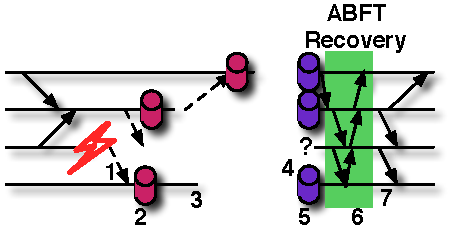
\includegraphics[width=.45\linewidth]{figures/idea.pdf}} \\
		1. MPI returns an error on surviving processes &  \\
		2. Surviving processes checkpoint & \\
		3. Surviving processes exit & \\
		4. A new MPI application is started & \\
		5. Processes load from checkpoint (if any) & \\
		6. Processes enter \abft dataset recovery & \\
		7. Application resumes & \\
		& \\
		\hline
	\end{tabular}
\end{table}

Based on the capabilities of the current version of the MPI Standard, we
designed a new approach for supporting \abft applications, called
Checkpoint-on-Failure (\cof). Table~\ref{tab:cof:cof} presents the steps
involved in the \cof method. In the figure, horizontal lines represent the
execution of processes in two consecutive MPI applications. When a failure
eliminates a process, other processes in the application are notified and regain control from
ongoing MPI calls (1). Surviving processes should assume the MPI library is
dysfunctional and not continue to use MPI operations (in particular, they do
not yet undergo \abft recovery). Instead, they checkpoint their current state
independently (2) and abort (3). If any processes were not initially alerted to
the failure, they will eventually be notified after the cascading calls to
\mpifunc{MPI\_ABORT} reach one of their neighbors. When all processes have exited,
the job is usually terminated, but the user (or a managing script, batch
scheduler, runtime support system, etc.) can launch a new MPI application (4),
which reloads processes from checkpoint (5). In the new application, the MPI
library is functional and communications are possible; the \abft recovery
procedure is called to restore the data of the process(es) that could not be
restarted from checkpoint (6). When the global state has been repaired by the
\abft procedure, the application is ready to resume normal execution (7). If another
failure hits the system during the recovery, the local states are not updated,
and the relaunch starts from the beginning. If another failure hits the system
after the \abft recovery, the entire procedure is followed to handle it.

\cof is most directly comparable to the existing method of periodic checkpointing.
Compared to periodic checkpointing, in \cof, a process pays the cost of creating
a checkpoint only when a failure, or multiple simultaneous failures, have
happened, hence it creates an optimal number of checkpoints during the run (and
no checkpoint overhead on failure-free executions). Moreover, in periodic
checkpointing, a process is protected only when its checkpoint is stored on
safe, remote storage, while in \cof, local checkpoints are sufficient: the
forward recovery algorithm reconstructs datasets of processes which cannot
restart from a checkpoint. Of course, \cof also exhibits the same overhead as
the standard \abft approach: the application might need to do extra computation,
even in the absence of failures, to maintain internal redundancy (whose degree
varies with the maximum number of simultaneous failures) used to recover data
damaged by failures. However, \abft techniques often demonstrate excellent
scalability; for example, the overhead on failure-free execution of the \abft QR
operation (used as an example in Section~\ref{sect:cof:cofqr}) is inversely
proportional to the number of processes.

\section{MPI Requirements to support \cof}\label{sect:cof:mpi}

To support \cof, some demands are made of the underlying MPI implementation.

\paragraph*{Returning Control After Failures:} Many MPI implementations not only
choose \mpifunc{MPI\_ERRORS\_ARE\_FATAL} as the default MPI error handler, but also
either do not implement the ability to choose another error handler, or provide
other error handling mechanisms which supercede the MPI error handlers. For \cof
to be functional, the MPI implementation must provide a functional error
handler mechanism, including \mpifunc{MPI\_ERRORS\_RETURN} as well as custom
error handlers defined by the application. In addition, the MPI implementation
must guarantee that after a failure, it returns control to the application by
invoking the error handler. It does not need to provide a perfect failure
detector~\cite{Fischer:1985tt} where all processes are immediately notified of failures (indeed, that
is often the wrong type of failure notification due to its high overhead cost), 
but it must never deadlock because of a failure, preventing the application from 
regaining control and performing recovery mechanisms, defined as an eventually perfect failure detector.

\paragraph*{Termination After Checkpointing:} The application must be able to
reliably ensure that all other processes are notified of the failure after any
process detects it. This can be through a user-controllable mechanism, such as
exiting without calling \mpifunc{MPI\_FINALIZE} or by invoking
\mpifunc{MPI\_ABORT}, but if the failure is not propagated, then some processes
will take a recovery execution path while others attempt to continue normal
execution and eventually reach a deadlock scenario.

\section{Open MPI Implementation}\label{sect:cof:ompi}

Open MPI is an MPI 2.2 compliant implementation of the MPI standard.
Architecturally, it is divided into two main levels: the runtime (ORTE) and the
MPI library (OMPI). As with many MPI implementations, the default behavior of
the library is to abort upon process failure. This policy was implemented deeply
at the runtime layer, preventing the OMPI layer from making any policy decisions
on the status of the library after a failure. To correct this, major changes
needed to be implemented in ORTE.

\subsection{Resilient Runtime}\label{subsect:cof:ompi:resilient}

The main contribution of the Open MPI runtime is to provide process management.
This includes creating new processes at the beginning of an MPI job, cleaning up
processes at the end of the job, and spawning new processes within the job if
requested by the application. To accomplish this task, ORTE includes an
out-of-band (OOB) communication mechanism which allows the ORTE layers to
communicate amongst each other without impacting the performance of the high 
performance network. When a node failure occurs, not only is the application's 
communication ability impacted, but also the runtime. ORTE needs to be able to react and repair
the OOB communication topology to route around failures and allow itself to
continue process management. For some communication topologies, such as a star 
where all processes are directly linked to the head node,
this is a trivial operation and only requires excluding any failed processes
from the routing tables. For more elaborate topologies, such as a binomial tree,
the self-healing operations are more complex, requiring each node to recompute
the tree around it to repair any links. If a parent process in the tree fails,
the healing process needs to make a new link to the next alive process
traveling up the tree. If a child process fails, the same needs to happen
traveling downward. In this way, the tree will always remain connected among
alive processes. However, it is not guaranteed, and indeed unlikely, that the tree
will remain balanced. It was determined that this was not a critical requirement
of the OOB as it is not used as a high performance messaging layer in Open MPI,
only as a communication mechanism for process management.

\subsection{Failure Notification}\label{subsect:cof:ompi:notification}

In addition to providing a self-healing OOB communication mechanism to
facilitate \cof, ORTE also needed to provide basic failure notification. To
track the status of failures, an incarnation number has been added to the ORTE
process names. When a failure is detected, the name of the failed process
(including its incarnation number) is broadcast over the OOB topology. The
incarnation number provides a mechanism to determine which process failures are
already known and which are not, preventing duplicate recoveries for the same
process failure. It also prevents a transient process failure from causing
confusion among the processes in the OOB by ensuring that all processes know
with which incarnation of a particular process they should be communicating. To
propagate this knowledge, ORTE processes monitor the health of their neighbors
in the OOB topology. When a failure is detected, the processes around the failed
process perform the route healing described in \ref{subsect:cof:ompi:resilient}
followed by a reliable broadcast algorithm which informs all processes in the
application of the failure. This algorithm has a low probability of creating a
bifurcation of the routing topology. Indeed, in the provided OOB topologies, 
this algorithm will never produce a bifurcation. On each node, when the ORTE 
layer is notified of process failure, it forwards the information to the OMPI 
layer, which has been modified to invoke the appropriate MPI error handler, as 
determined by the user.

\section{Example: QR-Factorization using \cof}\label{sect:cof:cofqr}

This section illustrates the usefulness of \cof by demonstrating its applicability to a
widely used class of algorithms: dense linear factorizations. The linear algebra
algorithm modification performed in this section was done by Peng Du building on the \cof library we
implemented. The QR factorization is a cornerstone in many applications,
including solving $Ax = b$ when matrices are ill-conditioned, computing
eigenvalues, least square problems, or solving sparse systems through the GMRES
iterative method. For an $M \times N$ matrix $A$, the QR factorization produces
$Q$ and $R$, such that $A = QR$ and $Q$ is an $M \times M$ orthogonal matrix and
$R$ is an $M \times N$ upper triangular matrix. The most commonly used
implementation of the QR algorithm on a distributed memory machine comes from
the ScaLAPACK linear algebra library~\cite{dongarra1997scalapack}, based on the
block QR algorithm. It uses a 2D block-cyclic distribution for load balancing,
and is rich in level 3 BLAS~\cite{Dongarra:1990wl} operations, thereby achieving
high performance.

\subsection{ABFT QR Factorization}\label{subsect:cof:cofqr:abft}

In previous work~\cite{pengduppopp12}, the QR factorization algorithm written 
for ScaLAPACK was modified to include \abft techniques, leveraging FT-MPI as the 
platform to maintain MPI communication after a failure. To ensure that the data 
in both the left ($Q$) and right ($R$) factors is protected from fail-stop 
errors during execution, a technique called Reverse Neighboring Checksum Storage 
is used. For each group of ($Q$) processes, a checksum and a duplicate are 
calculated and stored at the end of the matrix as shown in 
Figure~\ref{fig:cof:checksum}. These checksums are automatically updated 
as the algorithm is executed. The matrix-matrix multiplication which updates the 
right side of the original matrix will also update the values of these 
checksums. Because of this property, the more expensive checksum operation is 
absorbed by the already executing DGEMM kernel.

\begin{figure}
	\centering
    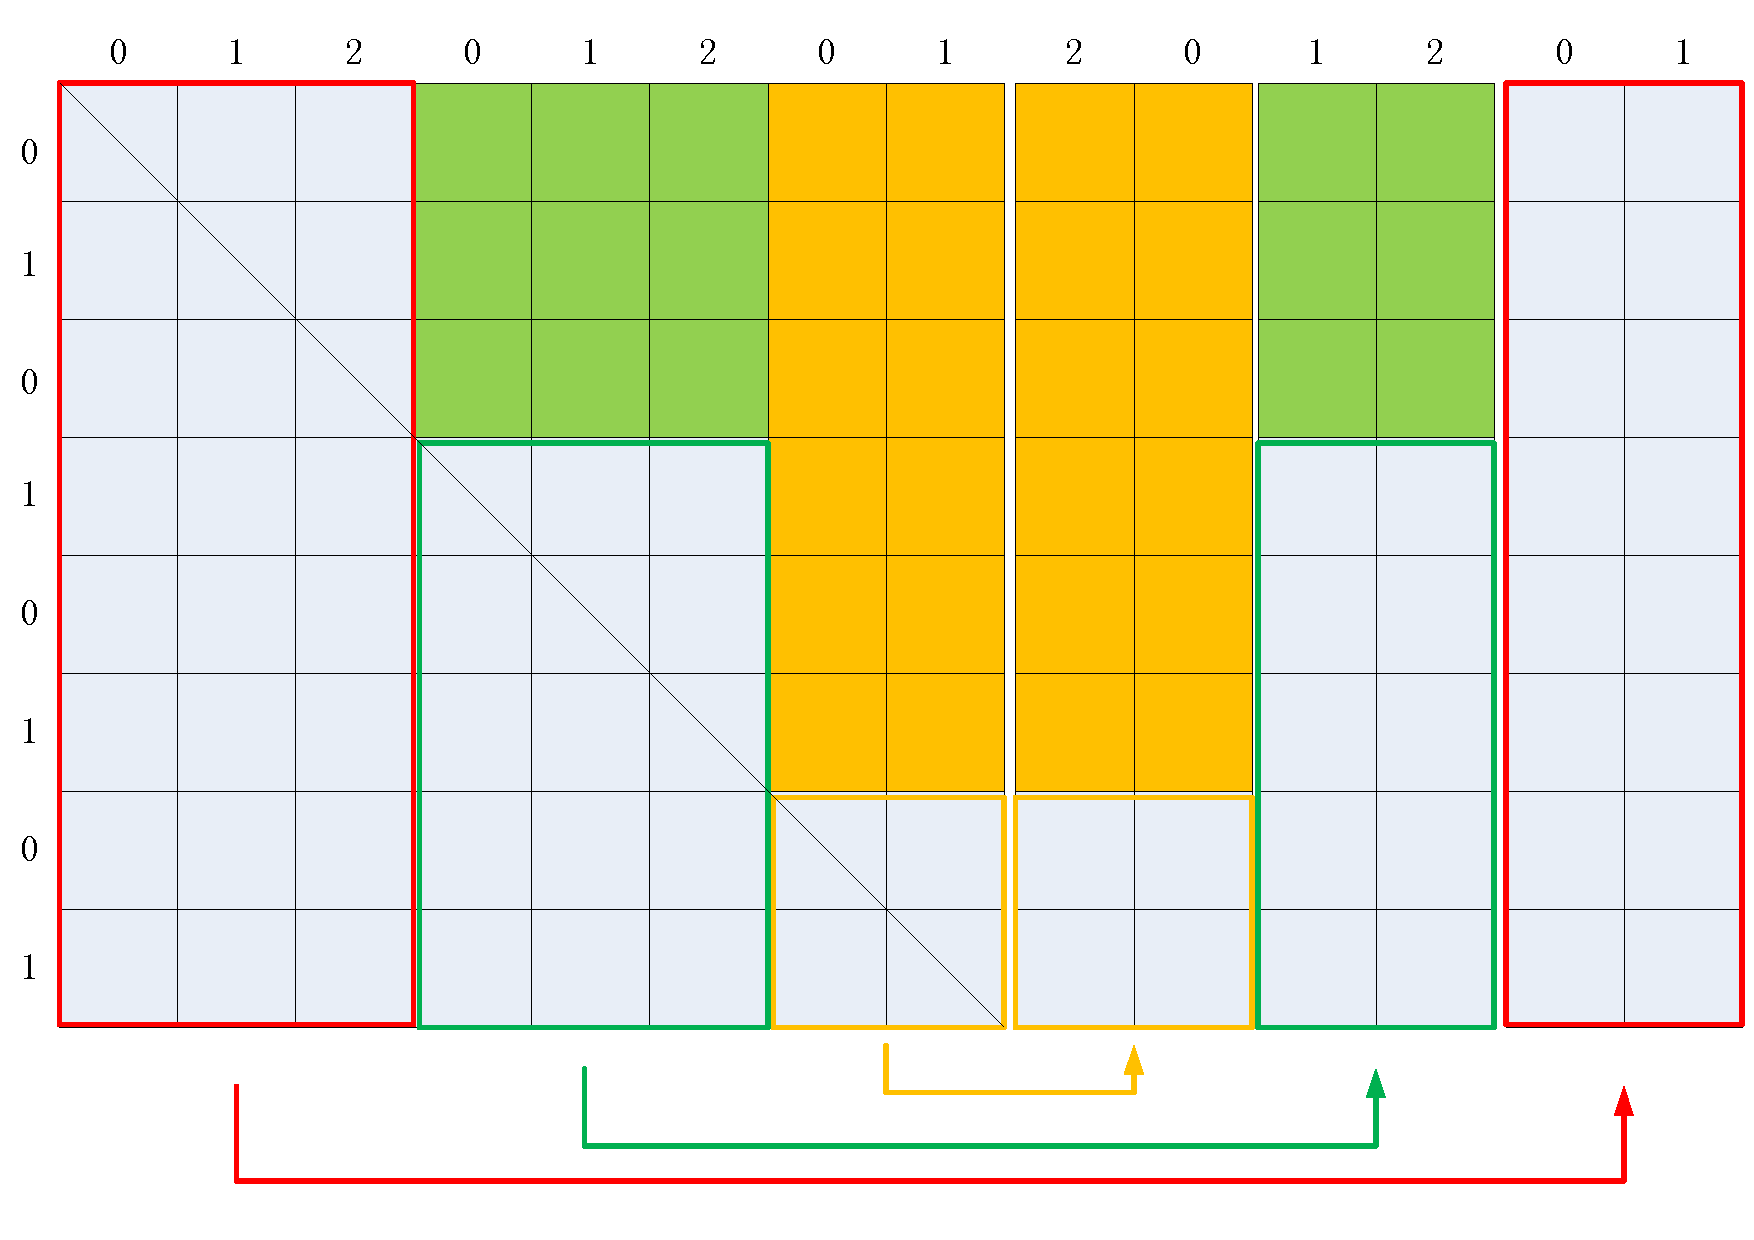
\includegraphics[width=.8\linewidth]{figures/hybrid-chpt-2x3}
    \caption{Pattern to store checksums to prevent data loss in the event of multiple failures. Figure borrowed from~\cite{pengduppopp12}}.
    \label{fig:cof:checksum}
\end{figure}

When a process failure is detected, all remaining processes are alerted of the 
location of the failure by FT-MPI, which creates a replacement process in the 
same coordinates in the $P \times Q$ block-cyclic distribution as the failed 
process. To restore any missing checksums, the value is simply copied from a 
duplicate. To restore the missing data blocks within the right factor of the 
matrix, a reduction operation calculates the value of the missing data by 
subtracting the remaining data values from the checksum. The value of the left 
factor is also stored in a checksum at the bottom of the matrix. Those values 
are either recovered from the checksum similarly to the right factor, or the 
most recent panel is recomputed.

While this algorithm was successful using FT-MPI, as previously stated, FT-MPI 
does not remain a viable candidate for MPI fault tolerance in the future. The 
algorithm was ported to a more compliant version of MPI, Checkpoint-on-Failure, 
to demonstrate its feasibility on existing systems.

\subsection{Checkpoint-on-Failure QR}

\paragraph*{Checkpoint Procedure:} 
Compared to a regular fault tolerance tool, \cof is not a standard checkpointing 
procedure. Where system-level checkpoints save the contents of large sections of 
memory, whether the data is still useful or not, \cof applications should only 
checkpoint the most vital pieces of data that are either required for an 
application to resume, or are prohibitively expensive to recalculate at recovery 
time. This means that codes should refactor their existing checkpointing 
functions to save less data and store it in a different location (depending on 
the type of application and execution environment). For \cof-QR, the 
checkpointing function saves the local values of the matrices and the loop 
indices necessary to restart. All other data critical to the application can be 
regenerated quickly from these most important pieces.

\paragraph*{State Restoration:} 
ScaLAPACK programs have deep call stacks,
including functions from several software packages, such as
PBLAS~\cite{Choi:1995:PSP:898829}, BLACS~\cite{Dongarra:1991vn, Dongarra:1995uu}, LAPACK~\cite{Anderson:1990th} and BLAS~\cite{Choi:1996wy}.
In the previously existing FT-MPI version of the QR algorithm, regardless of
when the failure was detected, the current iteration of the algorithm needed to
be completed before processing the recovery procedure. This would ensure an
identical call stack on every process and that all processes had updated their
checksums completely. For the new \cof version of QR, failure must interrupt the
algorithm immediately, not completing the current iteration, because the MPI
library can no longer support the communication necessary to calculate the most
up to date checksums. While this has the potential to cause divergent call
stacks among the processes, because failure notification happens only in MPI and
the lower level procedures (BLAS, LAPACK, etc.) do not perform communication,
the data remains uncorrupted by failures.

To resolve the call stack issue, when restarted, every process undergoes a ``dry
run'' phase where the algorithm mimics the loop nests of the QR algorithm down
to the PBLAS level without actually applying modifications to or exchanging
data. When the algorithm reaches the original point of failure, the matrix content is
loaded from the checkpoint data and the algorithm is able to continue in the
same manner as before in the FT-MPI based code. The regular recovery procedure
is applied: the current iteration of the factorization is completed to update
all checksums and the dataset is rebuilt using the ABFT reduction.

\section{\cof Performance}\label{sect:cof:performance}

In this section, we use our Open MPI and ABFT modifications to evaluate the performance
of the \cof protocol. We use two test platforms. The first machine, ``Dancer,''
is a 16-node, development cluster in the Innovative Computing Laboratory at the 
University of Tennessee. All nodes are equipped with two 2.27GHz quad-core E5520
CPUs, with a 20GB/s Infiniband interconnect. Solid State Drive disks are used as
the checkpoint storage media. The second system is the Kraken supercomputer, a 
University of Tennessee owned machine, housed at Oak Ridge National Laboratory.
Kraken is a Cray XT5 machine, with 9,408 compute nodes. Each node has two
Istanbul 2.6 GHz six-core AMD Opteron processors, 16GB of memory, and are
connected through the SeaStar2+ interconnect. The scalable cluster file system
``Lustre'' is used to store checkpoints.

\subsection{MPI Library Overhead}\label{subsect:cof:performance:overhead}

One of the main concerns from application developers when discussing fault
tolerance is the amount of overhead introduced by the addition of fault
tolerance into any application code or intermediate libraries. Our
implementation of fault detection and notification is mostly implemented in the
non-critical ORTE runtime. Typical HPC systems feature a separated service
network (usually Ethernet based) and a performance interconnect; hence health
monitoring traffic, which happens in the OOB service network, is physically
separated from the MPI communications, removing the possibility of introducing
network jitter due to fault tolerance messages. In addition, changes to the MPI
functions are minimal: the same condition that previously triggered
unconditional aborts has now been repurposed to trigger error handlers. As
expected, no impact on MPI bandwidth or latency was measured.
The memory usage of the MPI library is slightly increased, as the incarnation
number doubles the size of the process names. However, this is negligible in
typical deployments.

\subsection{Failure Detection}\label{subsect:cof:performance:detection}

Critical to the functionality of \cof is the reliable and expedient detection of
process failures. The asynchronous failure notification described in
Section~\ref{subsect:cof:ompi:notification}, provides this failure detection. We
designed a micro-benchmark to measure failure detection time as experienced by
MPI processes. The benchmark code synchronizes with an \mpifunc{MPI\_BARRIER},
stores the reference time, injects a failure at a specific rank, and enters a
ring algorithm until the MPI error handler stores the detection time. The OOB
routing topology used by the ORTE runtime introduces a non-uniform distance to
the failed process, hence failure detection time experienced by a process may
vary with the position of the failed process in the OOB topology.

\begin{figure}[t]
    \centering 
    \subfigure[Linear OOB Routing]{
		\label{fig:cof:linear-oob}
		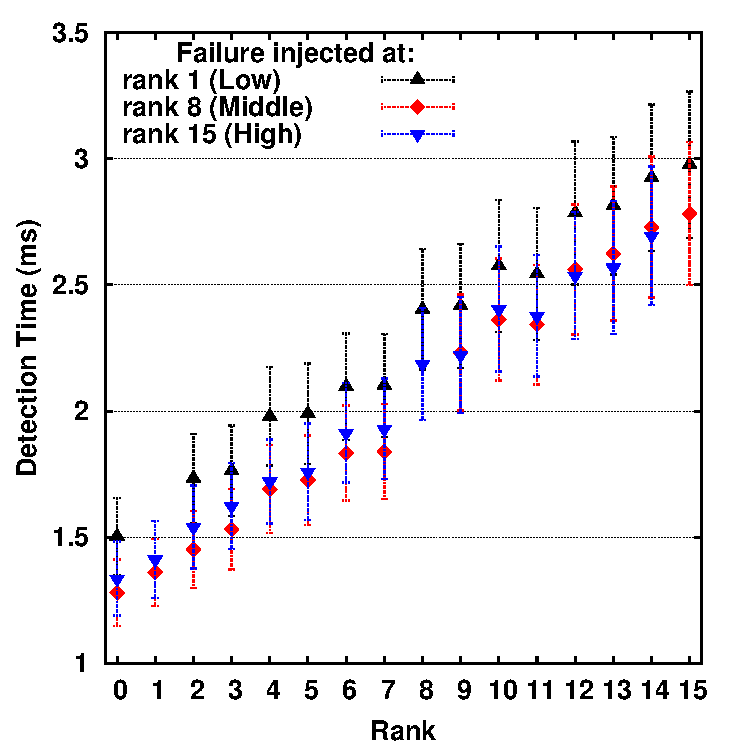
\includegraphics[width=.45\linewidth]{figures/failure-detection-linear-errbars}
	}
	\hfill
    	\subfigure[Binomial OOB Routing]{
		\label{fig:cof:binomial-oob}
    		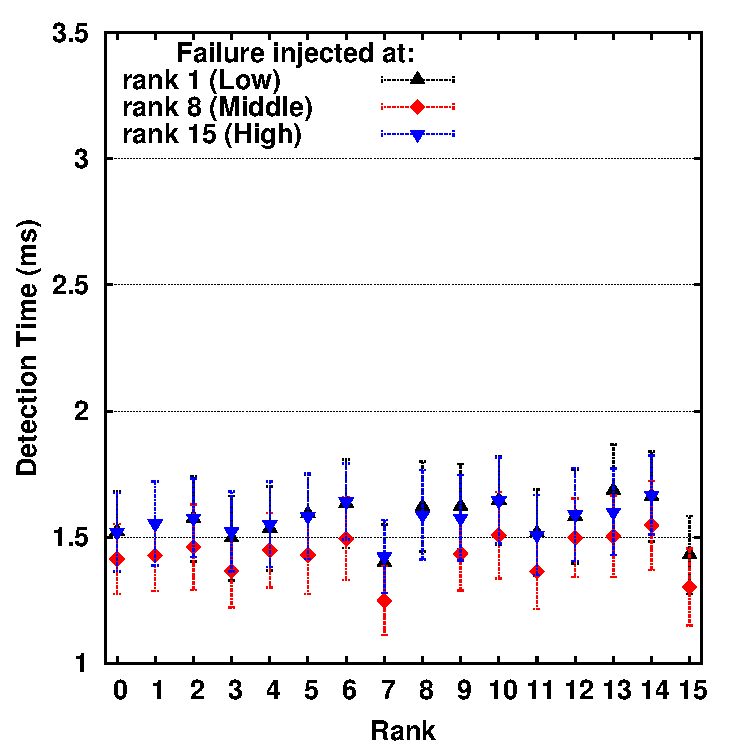
\includegraphics[width=.45\linewidth]{figures/failure-detection-binomial-errbars}
    	}
    \caption{Failure detection time, sorted by process rank, depending on the OOB 
    overlay network used for failure propagation.}
    \label{fig:cof:detection}
\end{figure}

Figures~\ref{fig:cof:linear-oob} and~\ref{fig:cof:binomial-oob} present the
failure detection times of the linear and binomial OOB topologies, respectively.
The curves ``Low, Middle, and High'' show the behavior for failures happening at
different positions in the OOB topology with ``Low'' failures being injected at 
rank 1, ``Middle'' failures occurring at rank 8, and ``High'' failures at rank 
15. On the horizontal axis is the rank of
the detecting process, and on the vertical axis is the detection time
experienced. The experiment uses 16 nodes, with one process per node, MPI over
Infiniband, OOB over Ethernet, an average of 20 runs, and the MPI barrier
latency is four orders of magnitude lower than the measured values.

In the linear topology (Figure~\ref{fig:cof:linear-oob}), every runtime process
is connected to the \emph{mpirun} process. For a higher rank, failure detection
time increases linearly because it is notified by the \emph{mpirun} process only
after the notification has been sent to all lower ranks. Obviously, this OOB 
topology is not designed to be a scalable solution. 

The binomial tree topology
(Figure~\ref{fig:cof:binomial-oob}) exhibits a similar best failure detection
time. However, this more scalable topology has a low output degree and
eliminates most contentions on outgoing messages, resulting in a more stable,
lower average detection time, regardless of the failure position. Overall,
failure detection time is on the order of milliseconds, a much smaller figure
than the typical checkpoint time.

\subsection{Checkpoint-on-Failure QR Performance}
\label{subsect:cof:performance:qr}

\begin{figure}[t]
    \centering
    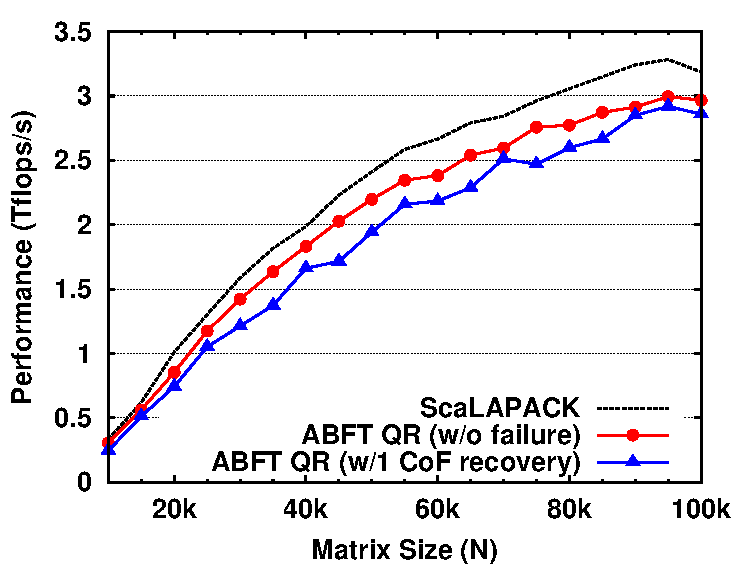
\includegraphics[width=.8\linewidth]{figures/kraken-new-data}
    \caption{ABFT QR and one \cof recovery on Kraken (Lustre).}%($24\times 24$ grid)
    \label{fig:cof:kraken-performance}	
\end{figure}

\paragraph*{Supercomputer Performance:} Figure~\ref{fig:cof:kraken-performance}
presents the performance on the Kraken supercomputer. The process grid is $24
\times 24$ and the block size is 100. The \abft QR (w/o failure) curve presents 
the performance of the \abft QR implementation, using \cof techniques, in a 
fault-free execution; it is noteworthy that when there are no failures, the 
performance is exactly identical to the performance of the unmodified \abft QR 
implementation with FT-MPI. The \abft QR (w/1 \cof recover) curve presents the 
performance when a failure is injected after the first step of the PDLARFB 
kernel. The performance of the non-fault tolerant ScaLAPACK QR is also presented 
for reference.

Without failures, the performance overhead compared to the regular ScaLAPACK is
caused by the extra computation to maintain the checksums inherent to the \abft
algorithm~\cite{pengduppopp12}; this extra computation is unchanged between
ABFT-QR without failures and ABFT-QR with a failure. Only on runs when a failure happened do the \cof protocols
undergo the supplementary overhead of storing and reloading checkpoints.
However, the performance of the \cof-QR remains very close to the no-failure
case. For instance, at matrix size N=100,000, \cof-QR still achieves 2.86
Tflop/s after recovering from a failure, which is 90\% of the performance of the
non-fault tolerant ScaLAPACK QR. This demonstrates that the \cof protocol
enables efficient, practical recovery schemes on supercomputers.

\begin{figure}[t]
	\centering
    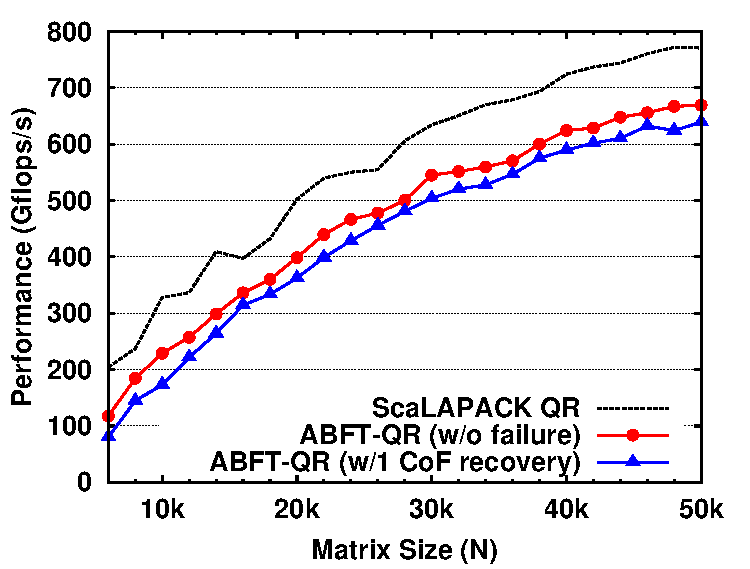
\includegraphics[width=.8\linewidth]{figures/dancer-performance-data}
    \caption{ABFT QR and one \cof recovery on Dancer (local SSD).}    	\label{fig:cof:dancer-performance}
\end{figure}

\begin{figure}[t]
	\centering
    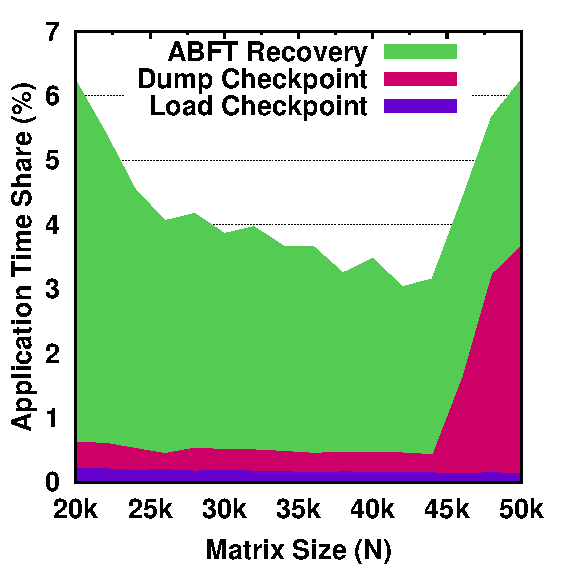
\includegraphics[width=.8\linewidth]{figures/dancer-1-error-timing-process-new-data}
    \caption{Time breakdown of one \cof recovery on Dancer (local SSD).}
    \label{fig:cof:dancer-timing}
\end{figure}

\paragraph*{Impact of Local Checkpoint Storage:}
Figure~\ref{fig:cof:dancer-performance} presents the performance of the \cof-QR
implementation on the Dancer cluster with an $8 \times 16$ process grid. Although
a smaller test platform, the Dancer cluster features local storage on nodes and
a variety of performance analysis tools unavailable on Kraken. As expected, the 
\abft method has a higher relative cost on this
smaller machine, but compared to the Kraken platform, the relative cost of \cof
failure recovery is smaller on Dancer. Like all algorithms involving 
checkpointing, the \cof protocol incurs disk access overheads to
store and load checkpoints when a failure hits, hence the recovery overhead
depends on I/O performance. By breaking down the relative cost of each recovery
step in \cof, Figure~\ref{fig:cof:dancer-timing} shows that checkpoint saving
and loading only take a small percentage of the total run-time, thanks to the
availability of solid state disks on every node. Since checkpoint reloading
immediately follows checkpointing, the OS cache satisfies most disk access,
resulting in high I/O performance. For matrices larger than N=44,000, the memory
usage on each node is high and decreases the available space for disk cache,
explaining the decline in I/O performance and the higher cost of checkpoint
management. Overall, the presence of fast local storage can be leveraged by the
\cof protocol to speedup recovery (unlike periodic checkpointing, which depends
on remote storage by construction). Nonetheless, as demonstrated by the
efficiency on Kraken, while this is a valuable optimization, it is not a
mandatory requirement for satisfactory performance.

\section{Evaluation of \cof}\label{sect:cof:evaluation}

Clearly, \cof does not meet all of the goals from Chapter~\ref{chap:goals}. It
provides relatively little \textbf{flexibility} due to the fact that it can only
write a checkpoint after discovering a failure. It does not provide a platform
to build other fault tolerance solutions. It provides sufficient \textbf{resilience} 
as it does allow the application to repair its execution by
reloading the data it writes after a failure. This allows the application to
continue executing even after a failure. Its greatest 
strength lies in its \textbf{productivity}. \cof is supported by existing MPI 
libraries and uses the familiar checkpointing paradigm as its basis. To that 
end, it is easily adopted by current applications as a possible solution for 
fault tolerance. A number of linear algebra algorithms can quickly adopt the tools in 
\cof with relatively little modification: one-sided factorizations, iterative conjugate 
gradient methods, and two-sided factorizations. The only changes necessary are to 
minimize the checkpoint size and to write a function to algorithmically repair the 
missing data. 

    \chapter{User Level Failure Mitigation}\label{chap:ulfm}

After creating \cof (see Chapter~\ref{chap:cof}), it became clear that designing
a fault tolerance framework within the existing MPI Standard to meet the goals
in Chapter~\ref{chap:goals} would not be feasible. At that point, we
investigated new ideas for fault tolerance that would require amendments to the
MPI Standard, and we created a proposal for a new chapter called User Level Failure
Mitigation. The complete document submitted to the \mpi Forum is provided in Appendix~\ref{chap:ft}.

\section{ULFM Design}\label{sect:ulfm:design}

Keeping with our design goals, we constructed a minimal set of new MPI
constructs which would provide the necessary changes to the MPI Standard to
allow applications to utilize fault tolerance in a way that makes sense to each
one individually, rather than defining a uniform recovery mechanism. To provide additional capabilities and conveniences, we encourage the creation of libraries (see Chapter~\ref{chap:apps}).

\subsection{Failure Reporting}\label{sect:ulfm:design:reporting}

Failure reporting is essential for fault tolerance. Applications must be
informed of failures from the MPI library in a consistent and predictable way in
order to construct recovery mechanisms. The alternative would cause the application 
to be aware of some failures and oblivious to others, leading to a deadlock 
between processes. To that end, we decided to report
failures using the return codes from existing MPI operations. This has the
double benefit of being easy to understand from an application perspective and
compliant with existing MPI constructs. Applications need only ensure that they
check return codes for all MPI operations and act appropriately, an action
which, ideally, they should already be taking, but in practice is not the current
standard procedure.

The fundamental error code that applications will receive to be alerted to a
process failure is \mpifunc{MPI\_ERR\_PROC\_FAILED}. Another error code will be
introduced later. When an application receives an error code related to a
process failure, it indicates that the operation could not be completed
successfully because an error occurred on one of the processes involved in the
operation. This definition was specifically crafted to convey two ideas: 1) if 
an error causes a failure which prevents an MPI operation from completing for a
process, that process must return an error code to report the failure; 2) if the
operation \textit{can} complete despite the failure for any reason (the communication involved in the operation is already finished, the implementation was able to circumvent the impact of the failures, etc.), it should do so and return
no error code related to the process failure. Thus, knowledge of process
failures is not global, but is local to any process which receives an error code
indicating it.

Using local rather than global failure notification has substantial positive 
performance implications. Considering the alternative: if an error causes a 
failure, all MPI processes
must report the same return code to the application to ensure global knowledge
of the system. This forces each MPI operation to conclude with an agreement
operation to determine the success or failure of the operation on all other
processes. The current best known agreement algorithm has a runtime of
$O(nlog(n))$~\cite{Hursey-log-agreement}, which is a large amount of overhead to
add to all MPI operations, some of which currently exhibit a runtime of
$O(log(n))$. By only enforcing global knowledge when the user requires it, we bypass this increased overhead and keep the per-operation cost low.

\begin{figure}[t]
    \centering
    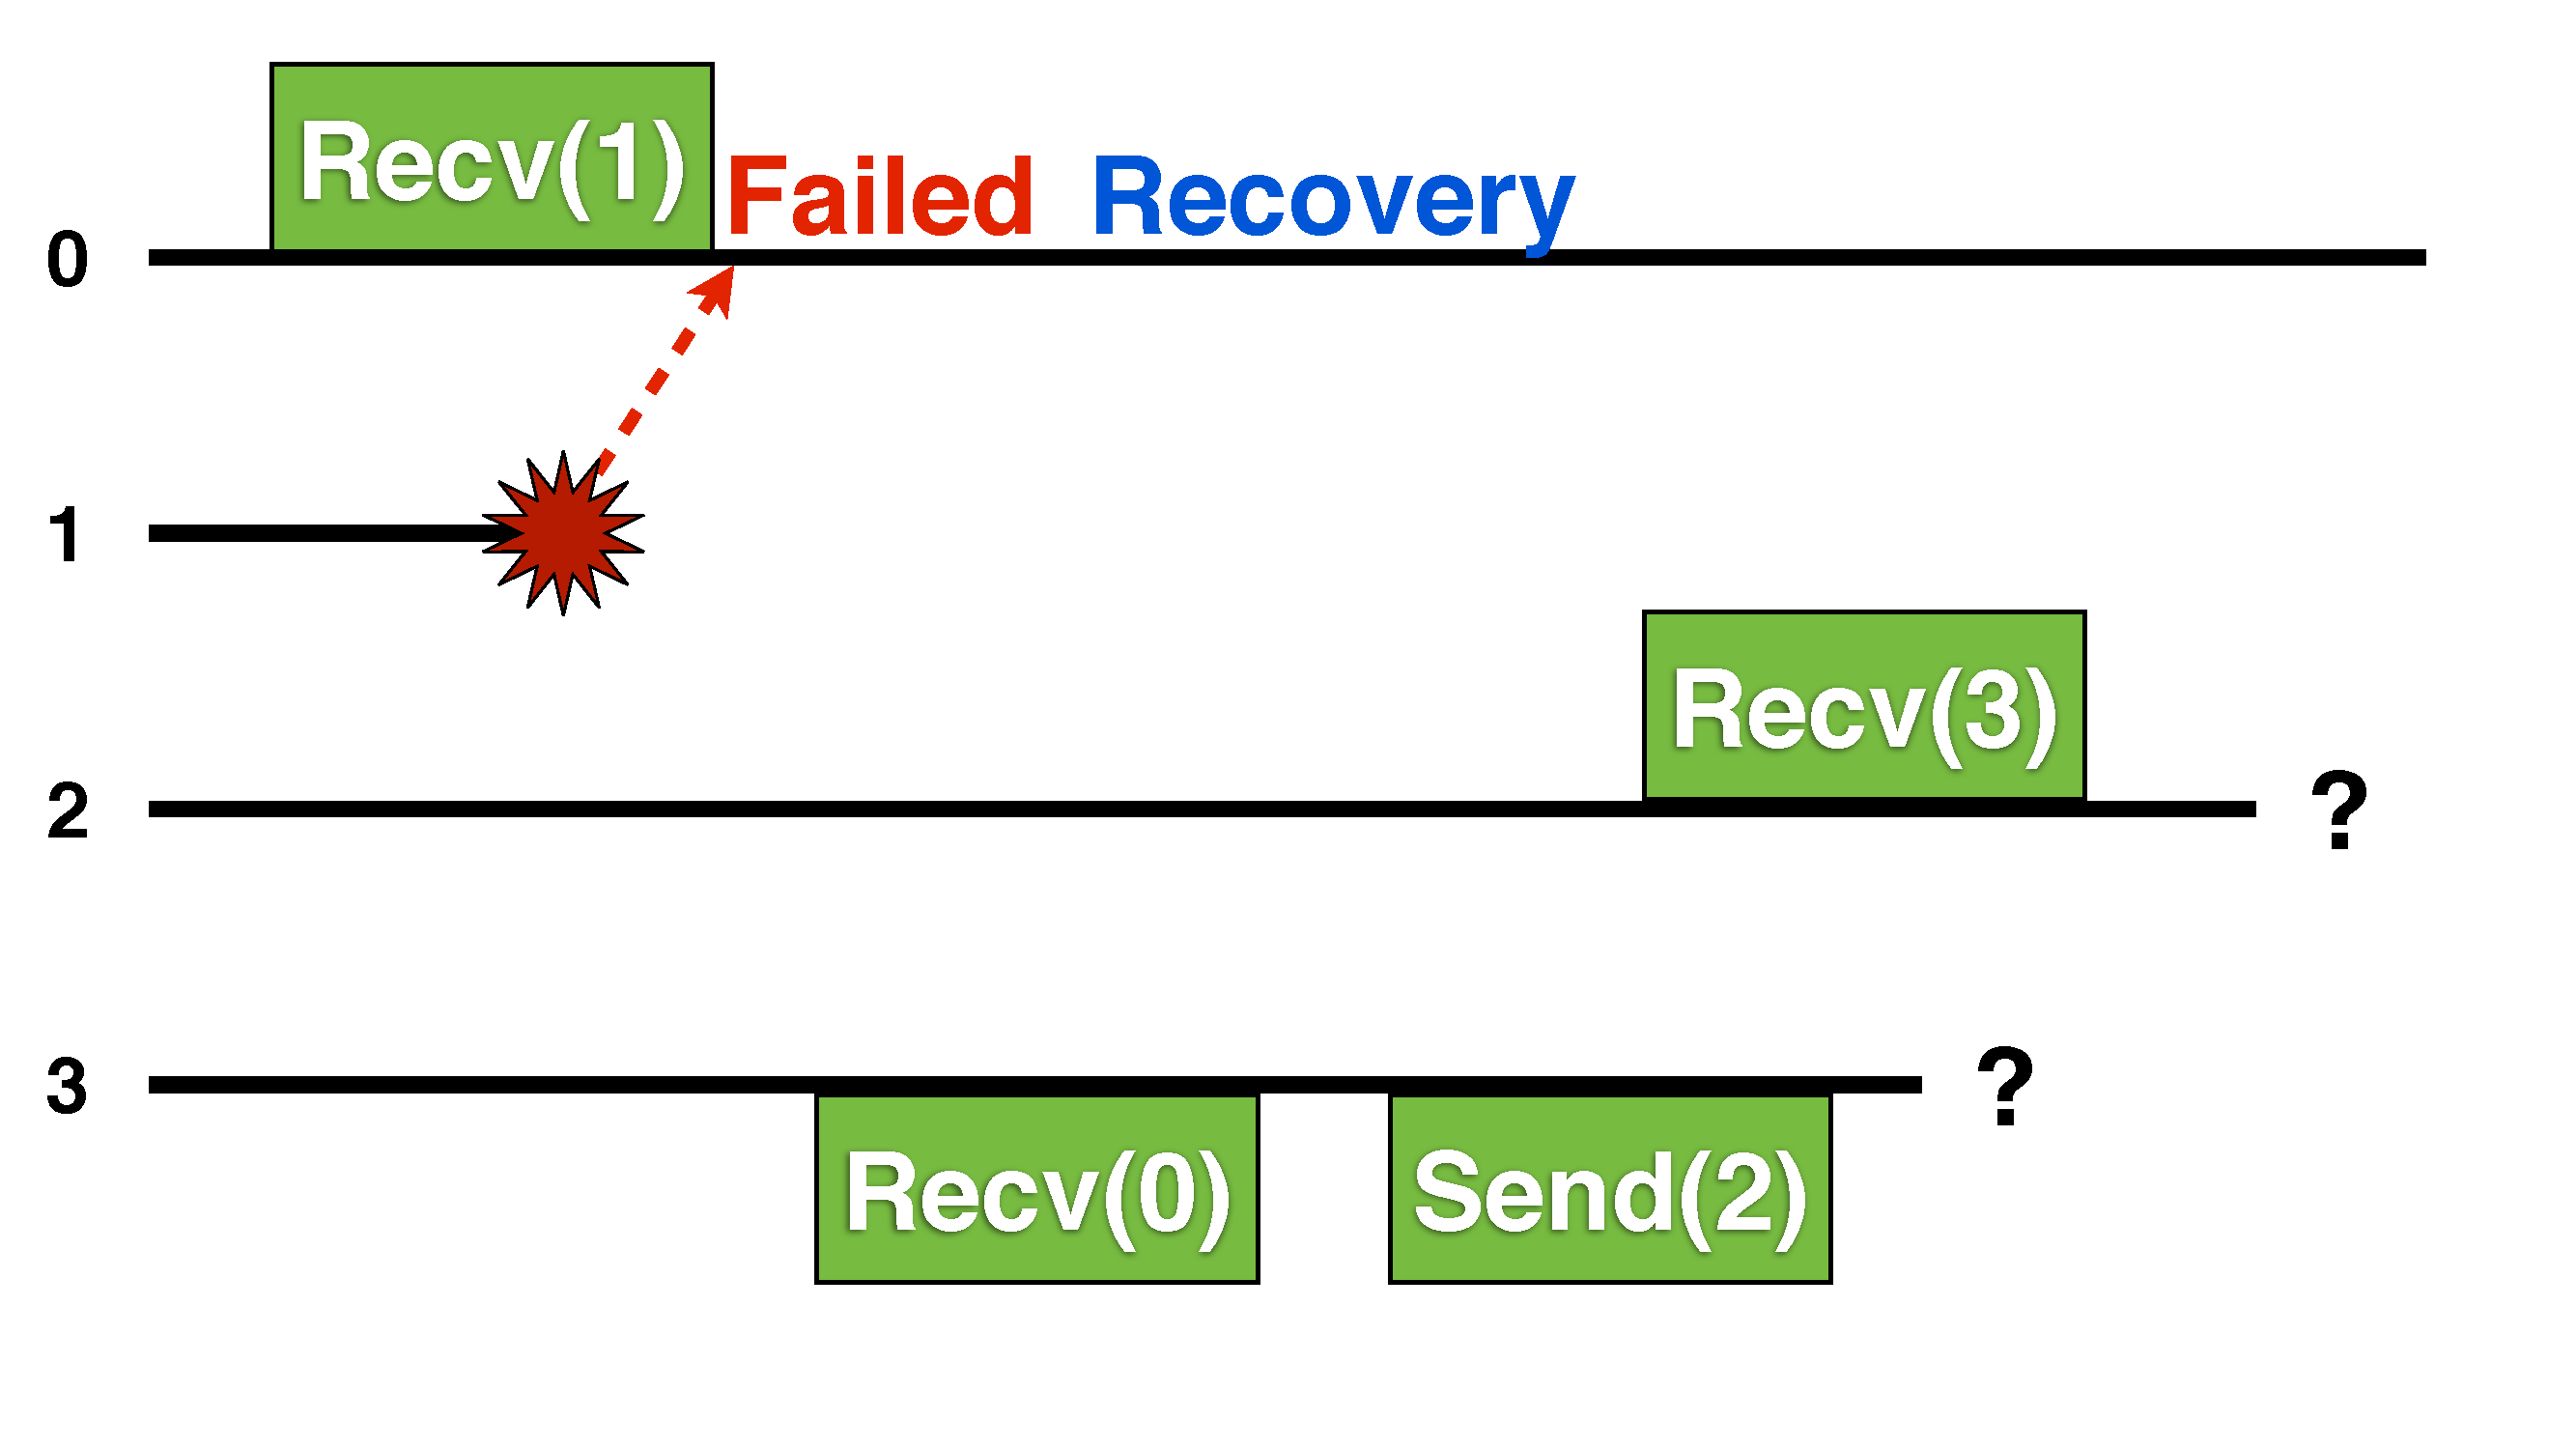
\includegraphics[width=\linewidth]{figures/NoRevoke}
    \caption{Application discovers failure and encounters deadlock}
    \label{fig:ulfm:no-revoke}
\end{figure}

Though it is now established that global knowledge of failure is expensive and
therefore should not be imposed on all applications, there are times where such
knowledge is necessary. The most obvious example of such a time is during
recovery. Figure~\ref{fig:ulfm:no-revoke} demonstrates an example of a recovery
situation where local knowledge is not sufficient to prevent deadlock. In this
example, four processes are communicating sporadically when process 1 fails.
Process 0 immediately discovers the failure because it is actively communicating
with process 1 at the time. Process 0 branches from the normal execution and
begins recovery operations. In the meantime, processes 2 and 3 are dependent on
communications from process 0 in order to continue their own execution. They
enter blocking operations where they become deadlocked. Because global knowledge 
of failures did not exist, the processes did not know to enter recovery 
operations or to cancel their outstanding communication operations and 
transition to recovery.

To resolve this situation, we introduce the new MPI construct:
\mpifunc{MPI\_COMM\_REVOKE}. This operation is a non-local, non-collective
operation to propagate failure information throughout an MPI Communicator. It
does this by using an out-of-band, resilient broadcast algorithm to interrupt 
all other non-local MPI operations and return the new error code
\mpifunc{MPI\_ERR\_REVOKED}. In this sense, it works similarly to the existing 
MPI function, \mpifunc{MPI\_ABORT}, without the subsequent ending of the MPI
application. Both \mpifunc{MPI\_ERR\_REVOKED} and the previously introduced 
error code, \mpifunc{MPI\_ERR\_PROC\_FAILED}, are permanent errors in the sense that once
one of these codes are returned, the MPI Communicator will never be usable again
for interprocess communication, though it is possible to transition from the
error code \mpifunc{MPI\_ERR\_PROC\_FAILED} to \mpifunc{MPI\_ERR\_REVOKED} after
the function \mpifunc{MPI\_COMM\_REVOKE} is called.

It is important to understand that \mpifunc{MPI\_COMM\_REVOKE} has no matching
call on remote processes. Once a process calls it on a particular MPI
Communicator, all other processes in the communicator will eventually receive
the notification of revocation through the error codes of other MPI operations
as if the function was called on their local processes. If another MPI process
never makes another call to an MPI operation, it will never be notified of the
revocation of the communicator. If it is necessary for all processes to be aware 
of process failures in this scenario, we provide a tool in 
Section~\ref{subsec:ulfm:consistency} to build such stronger consistency.

\begin{figure}[t]
    \centering
    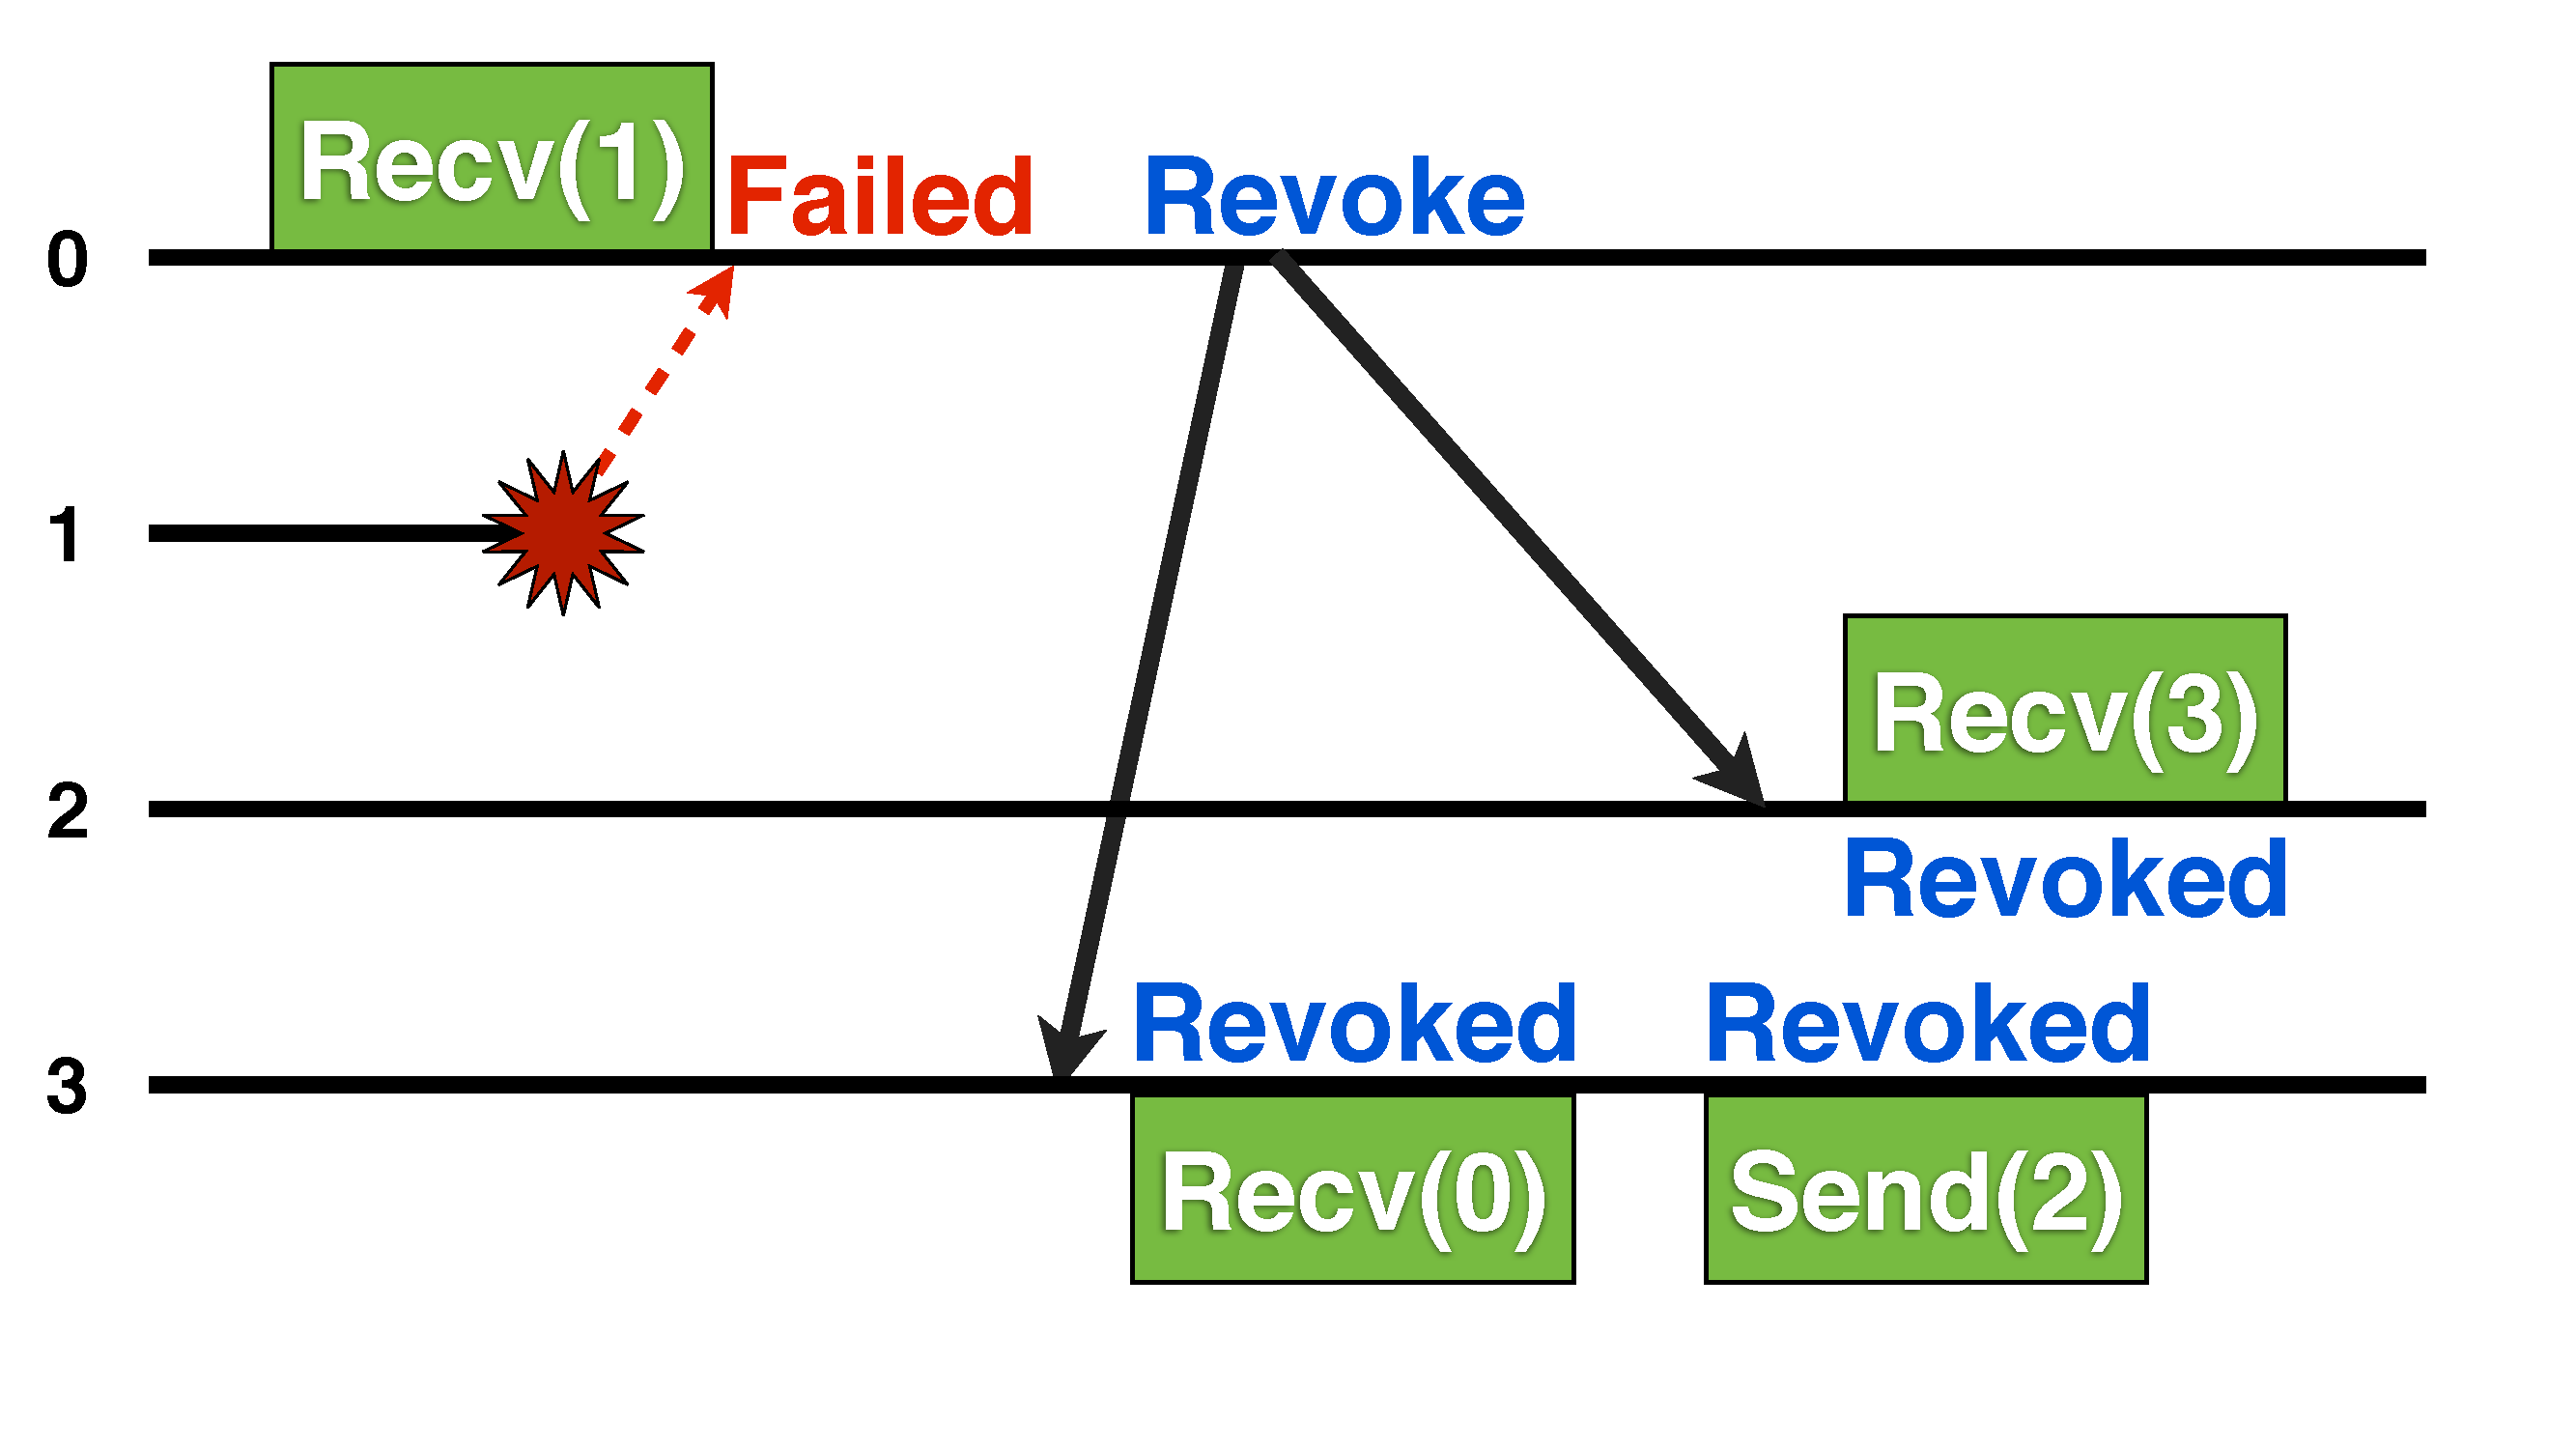
\includegraphics[width=\linewidth]{figures/Revoke}
    \caption{Application discovers failure and recovers using \mpifunc{MPI\_COMM\_REVOKE}}
    \label{fig:ulfm:revoke}
\end{figure}

By reexamining the scenario introduced earlier, now in
Figure~\ref{fig:ulfm:revoke}, we can see how this function might be used. After
the failure of process 1, process 0 invokes \mpifunc{MPI\_COMM\_REVOKE}.  While
processes 2 and 3 have already entered their respective communication
operations, the notification that their communicator has been revoked causes
those \mpifunc{MPI\_RECV} operations to return with the error code
\mpifunc{MPI\_ERR\_REVOKED}. At this point, all processes can perform recovery
together and the deadlock scenario in Figure~\ref{fig:ulfm:no-revoke} is averted.

Though \mpifunc{MPI\_COMM\_REVOKE} can appear to be a useful catchall tool to
introduce global knowledge of failures to all applications, a better
understanding of the tool emphasizes that it should be used carefully and only
in scenarios where it is required. Not all applications require global knowledge
of failures, and introducing it manually can impose a large synchronization and
recovery overhead that would be otherwise unnecessary. An example of such a
scenario is a Monte Carlo, master-worker style application. The usual
communication pattern of such applications is that all worker processes
communicate with a master process but not with each other. Thus, there are many
point-to-point communications, but no collective communications. These
applications should not use \mpifunc{MPI\_COMM\_REVOKE} to alert the worker
processes to failure of another worker, but should simply continue their point-to-point
communications unchanged. This example shows the flexibility of \ulfm by not
imposing an automatic recovery mechanism. In some cases, no recovery is the best
course of action.

% TODO - Sam stopped editing here. Give it a thorough reading.

\subsection{Rebuilding Communicators}\label{subsec:ulfm:rebuild}

When collective communication is required, using an existing MPI communicator
with failed processes is no longer an option. In this case, a new MPI construct
to restore the ability to communicate is necessary. To facilitate this, we
created the new function, \mpifunc{MPI\_COMM\_SHRINK}. This function is similar
to the automatic repair method of the same name used by FT-MPI~\cite{FaggFTMPI}. 
After an MPI communicator has been revoked, the remaining alive processes must 
call this function collectively. The shrink operation will create a new MPI 
communicator by executing an agreement algorithm among all alive processes to 
determine the group of processes which are believed to have failed. This failed 
group is excluded and a new MPI communicator is created with the remaining 
processes. The new communicator does not replace the revoked communicator, but 
is provided as a new MPI communicator with a new handle. This facilitates easier 
recovery by allowing the application to reference the previous ``version'' of 
the communicator to acquire information such as previous size, rank, and various 
other communicator properties.

Of all of the new MPI constructs, \mpifunc{MPI\_COMM\_SHRINK} was the most
difficult to design. Many options for communicator repair and recovery were
considered before deciding on shrink, some inspired by the recovery modes in
FT-MPI. We will mention some of the alternatives here to demonstrate the
rationale behind the design decisions.

\subsubsection{Blank}\label{subsubsec:ulfm:rebuild:blank}

The most seriously considered alternative to \mpifunc{MPI\_COMM\_SHRINK} was an
operation to replace failed processes with \mpifunc{MPI\_PROC\_NULL},
introducing blank positions within the MPI communicator. The advantage of this
scenario is that all processes retain their existing ranks and topologies,
making continuing execution after failure an easy transition as applications can
continue to communicate in the same patterns as before the process failure.
However, as with many of the communicator repair options, this mechanism does
not provide the flexibility seen in shrink. For example, by removing processes
from the communicator, they can no longer be queried to determine information
about the communicator, such as the ranks of the failed processes. This would also introduce a complexity when trying to replace the failed processes. These complexities will be further examined below.

\subsubsection{Replace}\label{subsubsec:ulfm:rebuild:replace}

Replace was the default recovery mechanism in FT-MPI. Failed processes were
automatically replaced with a new process in the same rank and location in the
MPI communicator. For applications, this is the simplest form of recovery to
understand because it automatically reconstructs \mpifunc{MPI\_COMM\_WORLD} and 
re-spawns failed processes. No manual recovery is required. However, from an
implementation perspective, implementing this automatic recovery mechanism is
very expensive and introduces many difficult problems related to communicator
reconstruction. FT-MPI solved the problem of communicator reconstruction by
destroying all communicators other than \mpifunc{MPI\_COMM\_WORLD} and requiring
the application to reconstruct the communicators manually. This is a
heavy-handed approach and is improved by using shrink. Also, as with the blank
functionality, using the replace mechanism does not facilitate as many other
forms of fault tolerance, but requires that applications conform to the
decisions mandated by replace.

\subsubsection{Using existing MPI functions}
\label{subsubsec:ulfm:rebuild:existing}

The last consideration was to modify the existing MPI functions to include
fault-tolerant semantics. An example of a function where this would make
sense is \mpifunc{MPI\_COMM\_DUP}. Semantically, the newly defined function
would be similar to \mpifunc{MPI\_COMM\_SHRINK}, however redefining existing MPI
constructs introduces both confusion and incompatibility. Existing MPI codes
would be forced to be rewritten to either specifically handle process failures
as defined by the new text or specifically exclude them, rather than the
behavior we chose where applications are clearly either using fault-tolerant
constructs, or are not, depending on whether or not they call the new recovery 
functions. Without very careful design, using existing functions as
fault-tolerant mechanisms could cause confusion if failures occur in an
inconvenient place. If a failure occurs just before \mpifunc{MPI\_COMM\_DUP} and
the operation creates the new communicator without the failed process, an
application which does not expect the recovery would need to perform extra
checks to see if the communicator has the expected size and composition. The 
same can be said for other MPI functions, such as the new function
\mpifunc{MPI\_COMM\_CREATE\_GROUP}, introduced by MPI-3.

\subsection{Failure Discovery}\label{subsec:ulfm:discovery}

\begin{figure}[t]
    \centering
    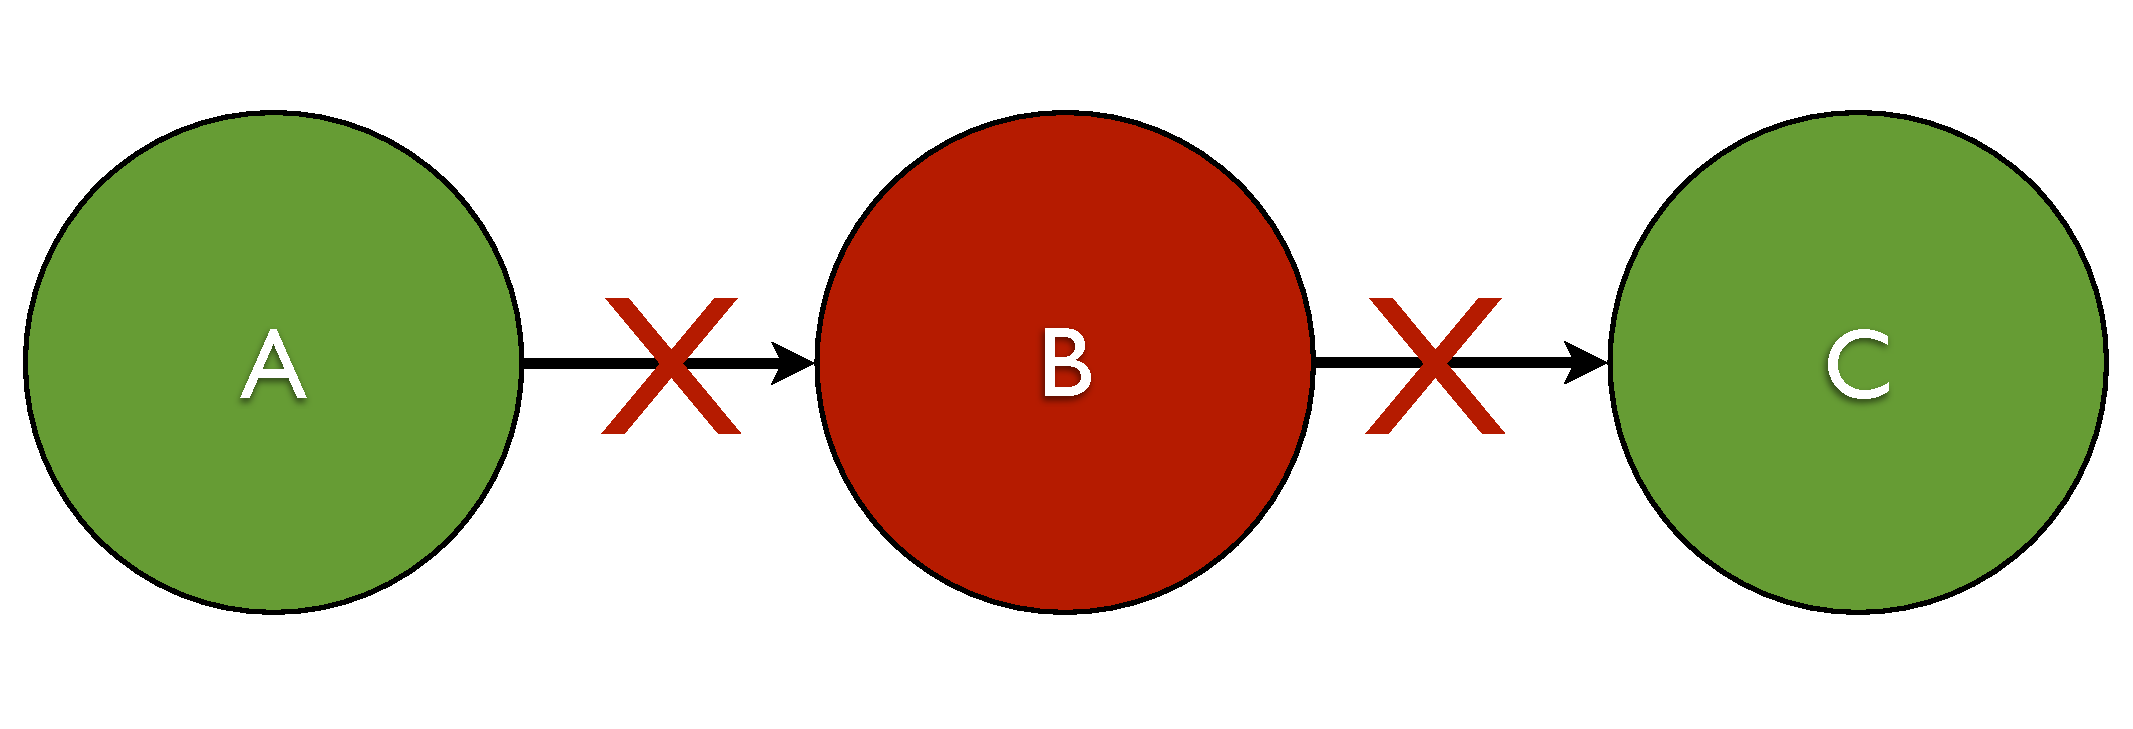
\includegraphics[width=\linewidth]{figures/intermediate-failure}
    \caption{Intermediate node failures report as
             \mpifunc{MPI\_ERR\_PROC\_FAILED}}
    \label{fig:ulfm:intermediate-failure}
\end{figure}

Once a failure has been reported to the MPI processes and the processes have
taken steps to disseminate knowledge as necessary, another issue must be
addressed. The living processes will need to have a mechanism to discover
which group of processes have actually failed and should be excluded from the
continuing application. While it might seem obvious that the failed process
would be the one with which the failed communication was taking place, this is
not guaranteed to be the case. As an example (see
Figure~\ref{fig:ulfm:intermediate-failure}), if process A is communicating with
process C and the communication topology routes messages through the node
containing process B, a failure of process B could result in an inability to
communicate between processes A and C. While a good MPI implementation should
make every effort to solve such routing issues transparently, it is possible
that a scenario would occur where such bifurcation is unavoidable or the
implementation chooses not to repair the communication paths. In this case, a
point to point communication operation between A and C would return the error
code \mpifunc{MPI\_ERR\_PROC\_FAILED}, even though neither A nor C has actually
failed. To discover the actual source of the failure, a new set of functions is
necessary.

The functions provided for this purpose are \mpifunc{MPI\_COMM\_FAILURE\_ACK}
and \mpifunc{MPI\_COMM\_FAILURE\_GET\_ACKED}. By calling this set of functions,
the application can acquire the \mpi Group containing the set of
processes which are known to have failed. \mpifunc{MPI\_COMM\_FAILURE\_ACK} sets
a reference point within the MPI implementation to which
\mpifunc{MPI\_COMM\_FAILURE\_GET\_ACKED} refers back when determining the group
of failed processes. This group represents only local knowledge and is not
guaranteed to be uniform among all process. No matter how many times the
\mpifunc{MPI\_COMM\_FAILURE\_GET\_ACKED} is called, the group of failed
processes will not change until the reference point is changed by calling
\mpifunc{MPI\_COMM\_FAILURE\_ACK}. By splitting the functions in two this way,
the application can maintain thread safety by controlling failure knowledge 
between the threads.

\subsection{Wildcard MPI Receive Operations}\label{subsec:ulfm:wildcard}

The other benefit of splitting the operation of acquiring the group of failed
processes into two functions is that the \mpifunc{MPI\_COMM\_FAILURE\_ACK}
function has another purpose. MPI contains a constant,
\mpifunc{MPI\_ANY\_SOURCE}, which can be used to specify that a receive
operation should match a message coming from any other rank within a
communicator rather than the usual format where a specific source is provided. 
When considering failure scenarios and knowledge of the status of
the ranks, this presents a difficult situation for the application. If a failure
needs to be reported during such a wildcard receive operation,
\mpifunc{MPI\_ERR\_PROC\_FAILED} is not an accurate representation of the status
of the operation. While a process involved in the operation will have failed, it
might not be the one with which the wildcard receive would have matched. In this
case, it is still important that we alert the application to a possible failure,
but we should also provide a way for the application to continue to use the
wildcard receive constant after the failure notification so as to not require an
expensive, complete recovery. In this situation, we return the error code
\mpifunc{MPI\_ERR\_PENDING} to inform the application that the receive operation
is still pending and can be completed after the application acknowledges the
failure using \mpifunc{MPI\_COMM\_FAILURE\_ACK}. Once the application
acknowledges the failure, the MPI library will not return another error code
related to that specific process failure and the application can re-enter the
wildcard receive operation. It should be noted that \mpifunc{MPI\_ERR\_PENDING}
is not a new error code, but the existing definition, ``pending request'', 
applies to this scenario and so defining a new error code was decided to be 
unnecessary.

\subsection{Process Consistency}\label{subsec:ulfm:consistency}

\begin{figure}[t]
    \centering
    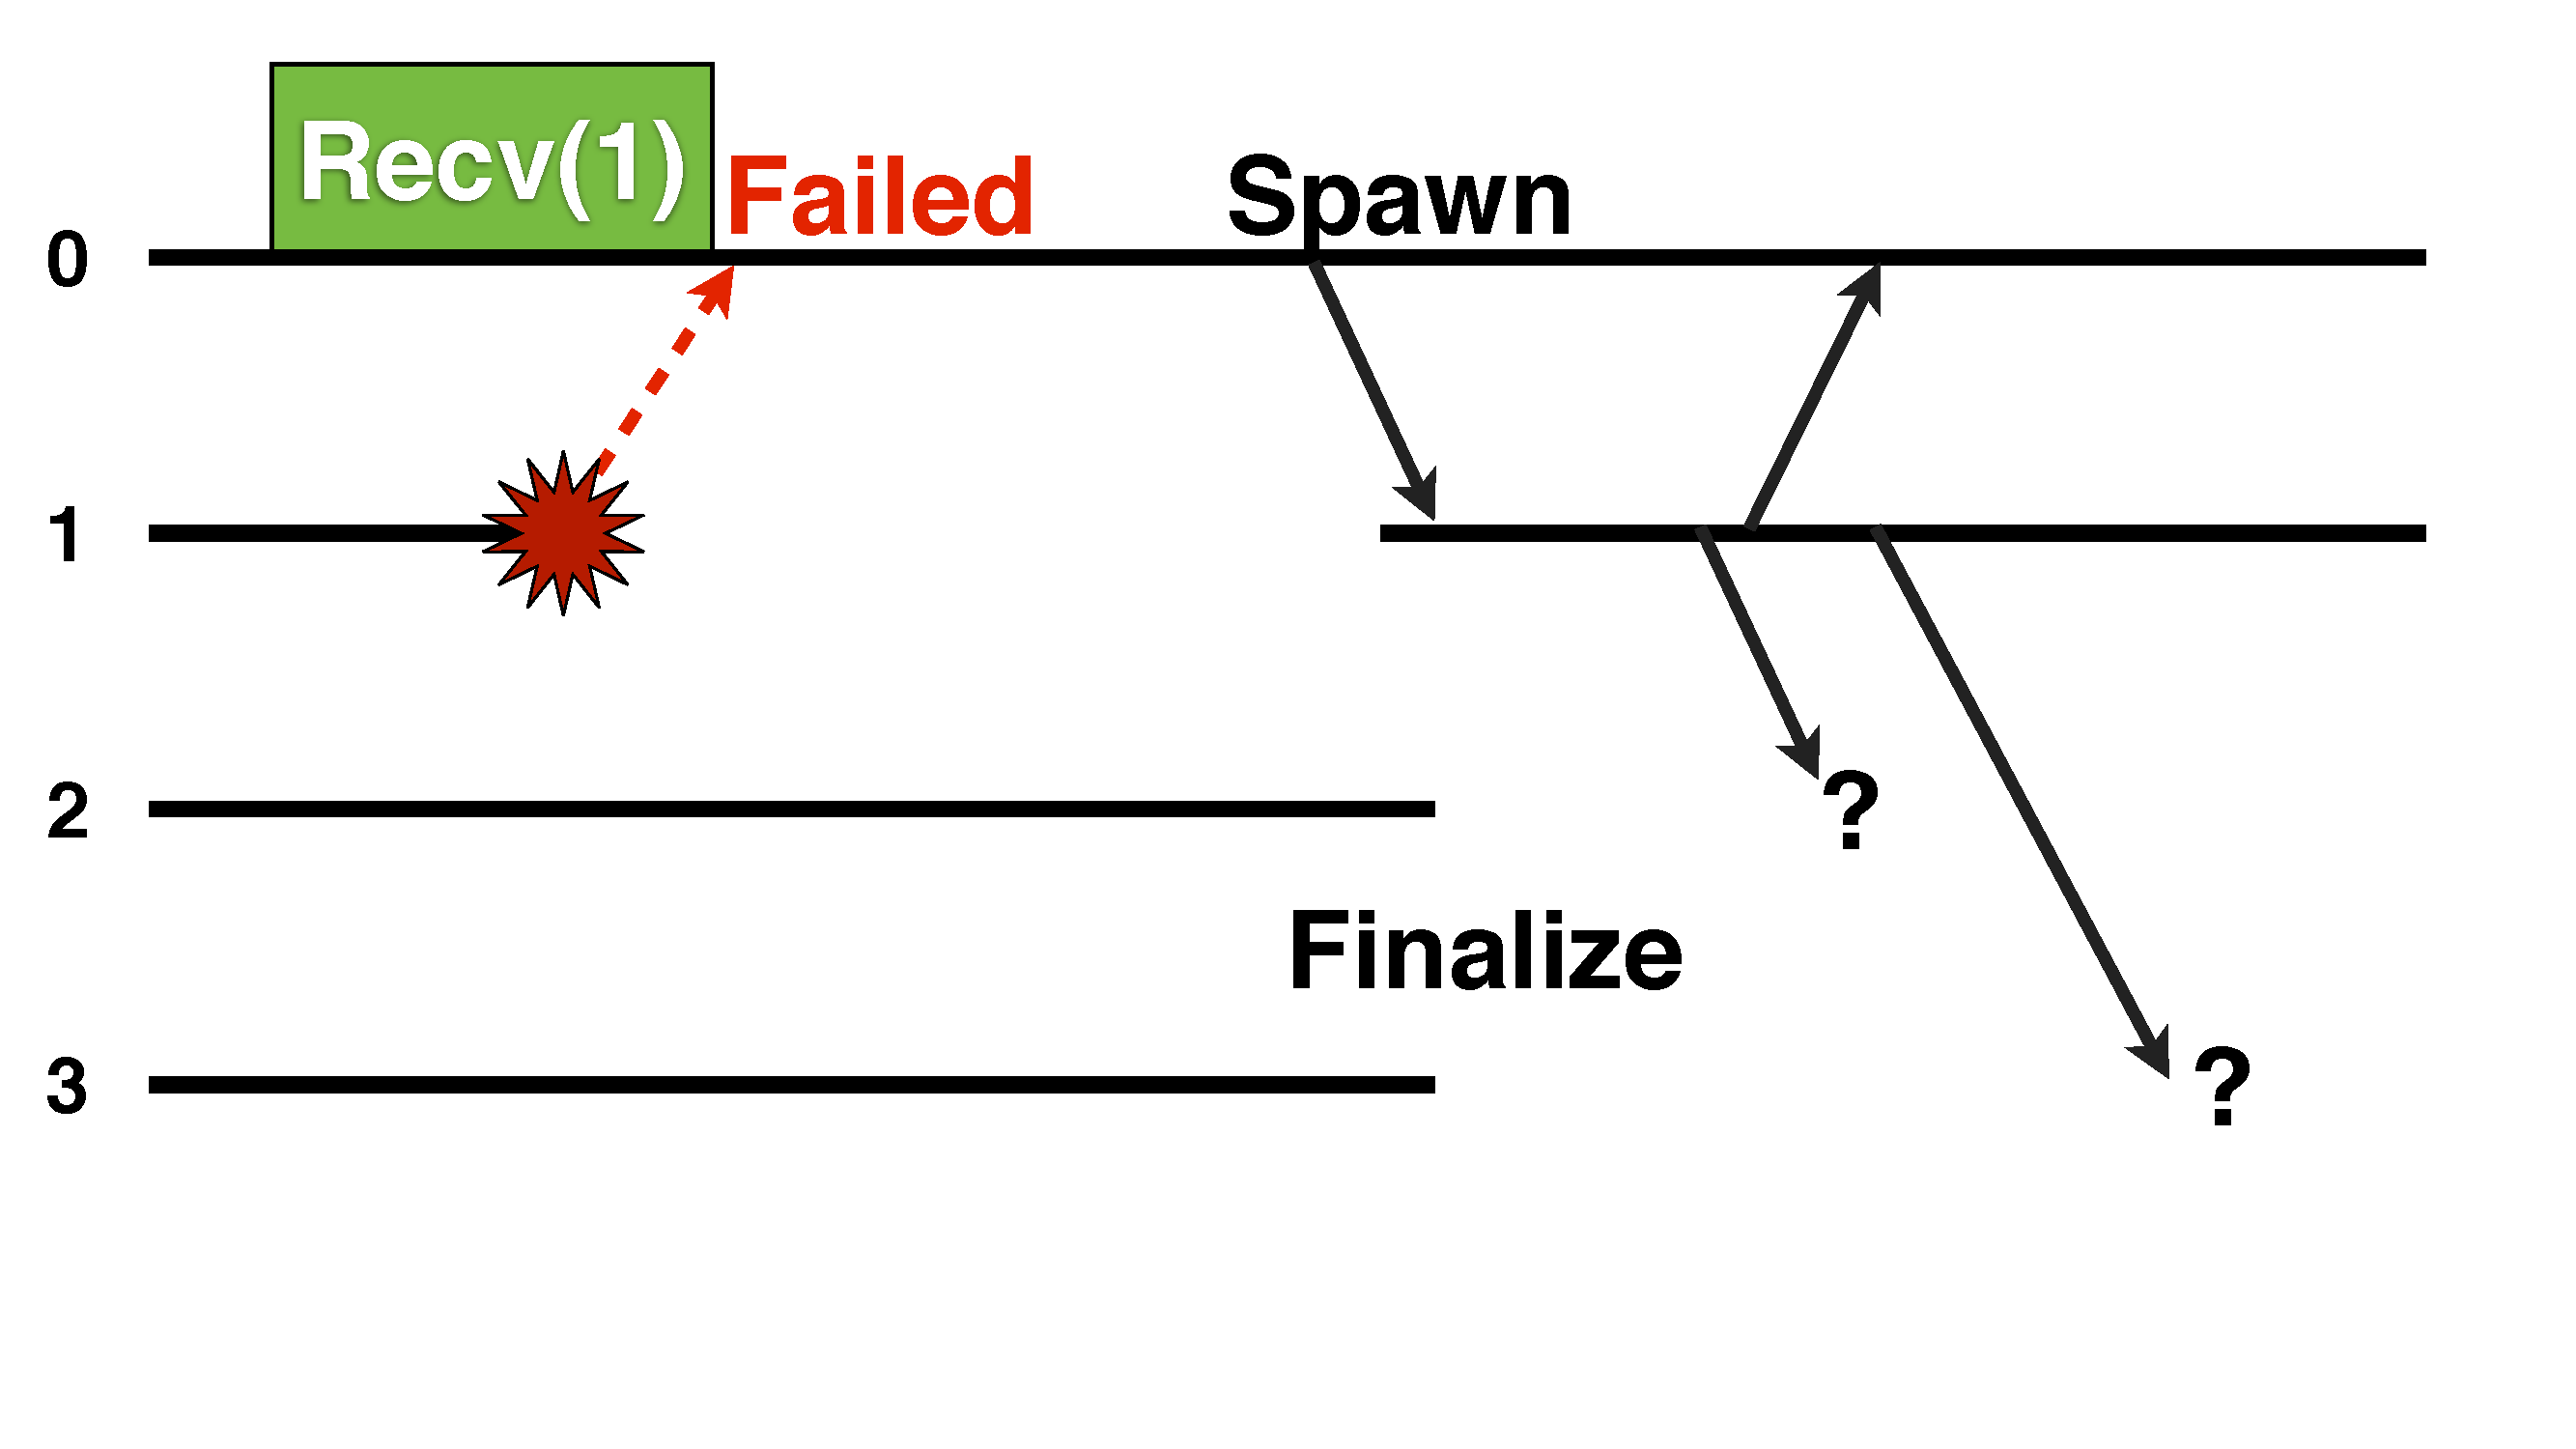
\includegraphics[width=\linewidth]{figures/NoAgree}
    \caption{Application reaches inconsistent state after some processes exit
             before other processes}
    \label{fig:ulfm:NoAgree}
\end{figure}

While a large focus of the ULFM work has been to provide a system with weak
consistency between processes to improve performance, there are times where
stronger consistency is necessary. Figure~\ref{fig:ulfm:NoAgree} demonstrates a
situation where this could occur. Processes 2 and 3 believe the application is
completed and call \mpifunc{MPI\_FINALIZE} while process 1 fails, to be
discovered by process 0. When process 0 spawns a replacement for process 1 and
the two processes try to perform recovery operations, the data needed from
processes 2 and 3 is no longer available. In this situation, an agreement
algorithm among the processes is necessary before algorithm completion to ensure 
that all processes successfully reach \mpifunc{MPI\_FINALIZE}. While in this scenario, using an
existing MPI function such as an \mpifunc{MPI\_ALLREDUCE} could solve the
problem, if the application does not need to recover process 1, the collective
operation would no longer complete successfully without repairing the
communicator, an expensive and possibly unnecessary operation.

To provide a tool to resolve this scenario, we created
\mpifunc{MPI\_COMM\_AGREE}. This function performs a fault tolerant agreement
algorithm over a boolean value among all alive processes. All alive processes
participate with the value passed in as an argument and all dead processes do
not participate (which is semantically equivalent to participating with the
value \textit{TRUE}). This allows applications which communicate only via point
to point operations to complete the agreement algorithm despite process
failures. The rationale behind ignoring process failures (including new process 
failures) is that if the failure
had impacted an MPI communication, that operation would have returned
an error code reporting the failure. If none of the processes detected that
failure, then it did not impact the results and can therefore be safely ignored.
If an error code was previously reported due to process failure, the process 
which received it can participate with the value \textit{FALSE} and all other 
processes will know that they need to enter recovery operations.

The only error code related to process failure that \mpifunc{MPI\_COMM\_AGREE}
may return is \mpifunc{MPI\_ERR\_REVOKED}. If the communicator has been revoked
remotely (or indeed locally), it is most likely that the revoke operation was
intended to interrupt even the finalization operation and that recovery is
necessary.

\section{Beyond Communicators}
\label{sec:ulfm:beyond}

While communicator operations are the most common use of MPI and historically
the core of MPI, there are other chapters of the MPI Standard that cover other
communication contexts. Dynamic processes, shared memory windows and collective 
file I/O operations have been included in the Standard to provide increased 
functionality in the form of one-sided communication operations and large scale 
file manipulation. The work to provide added fault tolerance capabilities to 
these types of operations will continue as this work was removed from the original proposal to the \mpi Forum, but the fundamentals detailed here are similar to the  fault tolerance designed for MPI Communicators.

\subsection{Failure Notification}
\label{subsec:ulfm:beyond:notification}

Well-defined failure notification is key to managing failures. By defining the
expected behavior of the MPI library after a failure, the application can design
resilience protocols to ensure a deadlock-free execution.

\subsubsection{Dynamic Processing}

Dynamic processing requires that the \mpi implementation construct new communicators, 
called intercommunicators, to connect the group of existing processes to the group of 
new processes. The most critical requirement is that if a process failure is detected 
while the MPI library is constructing the new MPI intercommunicator, the MPI 
library must always notify the root processes on either side of the 
intercommunicator. This is key because collective and point-to-point 
communication from the local group of an intercommunicator
to a remote group is expensive at best and impossible at worst after a failure has 
impacted the capabilities of the communicator. By ensuring the
root processes have been notified, they can provide notification to all 
processes in their local groups by revoking their communicator. Also, for 
similar reasons, when creating new processes by calling 
\mpifunc{MPI\_COMM\_SPAWN}, if a process failure is detected during the process 
or communicator creation, the MPI library should not return a partially 
constructed MPI communicator which cannot be repaired. Instead, the library 
should return a communicator that does not function (such as 
\mpifunc{MPI\_COMM\_NULL}) which will signify to the new MPI processes that they 
should probably abort, and to the old processes that they should attempt to spawn 
new processes again.

\subsubsection{One-Sided Communication}

One-sided communication operations behave as non-blocking communication 
operations. Because of this, they have similar failure notification definitions 
to calls involving MPI communicators such as \mpifunc{MPI\_ISEND} and 
\mpifunc{MPI\_IRECV}. Rather than notifying applications of process failure 
during the initialization calls, the library should delay notification to the 
one-sided completion calls (i.e. \mpifunc{MPI\_WIN\_COMPLETE}, 
\mpifunc{MPI\_WIN\_WAIT}, etc.). Remote memory access calls also have different 
failure semantics than traditional MPI communicator-based operations, though the 
motivation is similar. Whenever a failure is reported during one-sided epochs, 
the memory targeted during that period is undefined. This definition is similar 
to the fact that any buffers used during MPI operations where a failure is 
reported are also undefined. More specifics of the failure notification 
definitions for remote memory operations can be found in the specification 
document in Appendix~\ref{chap:ft}.

\subsubsection{File I/O}

File I/O operations are more complex when considering failure notification. 
Unlike communicator-based operations and one-sided communication operations, 
they usually do not involve synchronization calls which would facilitate failure 
propagation and notification. Because of this, after a failure the state of any 
open file pointers is left undefined. To help mitigate this indefinite result, 
users are encouraged to use a communicator which contains the same group of 
processes as those involved in an MPI file object to ensure that all processes 
remain functional after critical I/O calls. While this does create more overhead 
for file operations, it is less overhead than would be introduced by redefining 
the I/O operations to synchronize on each operation to ensure that all processes 
were successful.

\subsection{ULFM Functions for One-Sided Communication}
\label{subsec:ulfm:beyond:rma}

To assist with failure notification and recovery, two new functions have been
introduced for MPI one-sided communication. These functions closely mirror 
similar functions found in the communicator-based recovery 
Section~\ref{sect:ulfm:design}. 

The first function, \mpifunc{MPI\_WIN\_REVOKE} is
identical to \mpifunc{MPI\_COMM\_REVOKE}, but with MPI windows rather than MPI
communicators. When any process involved in a window calls \mpifunc{MPI\_WIN\_REVOKE},
all other processes are eventually notified by receiving the error code,
\mpifunc{MPI\_ERR\_REVOKED}. From this point on, all non-local operations
must continue to return the error code \mpifunc{MPI\_ERR\_REVOKED}. As with
\mpifunc{MPI\_COMM\_REVOKE}, this operation is both non-local and non-collective, 
meaning that if any process in the window calls the function, it impacts all other
processes without a matching call.

The second function, \mpifunc{MPI\_WIN\_GET\_FAILED} provides a mechanism to
retrieve the group of processes which are locally known to have failed at the 
time of calling. Note that this function is similar to the combined meaning of
\mpifunc{MPI\_COMM\_FAILURE\_ACK} and \mpifunc{MPI\_COMM\_FAILURE\_GET\_ACKED}.
The reason these functions are combined is that there is no need to acknowledge
the failure to allow wildcard operations to complete. One-sided communication
does not contain a similar operation.

\subsection{ULFM Functions for File I/O}
\label{subsec:ulfm:beyond:io}

As with failure notification, recovery functions for File I/O are also minimal.
The only function provided is \mpifunc{MPI\_FILE\_REVOKE}. Again, this function
is non-local and non-collective and will notify all other processes involved
in the MPI file and cause all subsequent non-local operations to return the
error code \mpifunc{MPI\_ERR\_REVOKED}.

When deciding whether to include a function to retrieve the failed processes 
from the file object, it was decided that a valid reference point to describe 
the failed processes does not exist. In communicators and windows, it is 
possible to retrieve the group of processes involved in the communication 
object. However, for file objects, this option is not available. This makes 
describing the failed processes difficult and the need for a function such as 
\mpifunc{MPI\_FILE\_GET\_FAILED} unnecessary.

% TODO - George stopped editing here

\section{ULFM in Applications}
\label{sec:ulfm:apps}

\ulfm has already been ported to some existing applications to demonstrate its 
usability in real-world scenarios. This section describes its use in the 
linear algebra \abft-QR algorithm detailed in Section~\ref{sect:cof:cofqr}.

\subsection{Example: QR-Factorization}
\label{subsec:ulfm:apps:qr}

This example is another proof of concept demonstration as in 
Section~\ref{sect:cof:cofqr}. The \abft algorithm for QR factorization is the 
same, but the recovery technique changes to incorporate the new capabilities of 
\ulfm. Rather than dumping the checkpoints to disk, restarting the MPI job, 
re-reading the data from disk, and continuing the execution, the \ulfm version of 
\abft-QR does not need to perform all the tasks to restart MPI. Instead, remaining 
processes can start a replacement for the failed process and perform forward 
recovery without needing to restart the existing MPI processes.

When a process failure is detected in the QR algorithm, an error is returned 
to the application. The application revokes the communicator being used by the 
BLACS (Basic Linear Algebra Communication Subroutines)~\cite{Dongarra:1995uu}
library to ensure that all processes are notified of the process failure (see 
the section on BLACS below for a description of the modifications to
BLACS to enable fault tolerance). After revoking the communicator with the failed 
process, the remaining processes create a working communicator using 
\mpifunc{MPI\_COMM\_SHRINK}. Using the new communicator, they spawn a new process 
to replace the failed process. By using \mpifunc{MPI\_INTERCOMM\_MERGE} and 
\mpifunc{MPI\_COMM\_SPLIT}, they can reposition the new process to have the same 
rank as the original process which it replaced. This means that the \abft 
algorithm can continue as before once the data recovery is complete.

\subsubsection{BLACS}
\label{subsubsect:ulfm:apps:qr:blacs}

BLACS is the intermediate library used by ScaLAPACK to abstract the communication in the linear algebra codes. While at one time it provided an abstraction for many 
communication libraries and platforms (MPI, PVM, HP Exemplar, IBM SP (MPI), Intel 
series (NX), and SGI Origin 2000 (MPI)), as most of these libraries have become 
unnecessary and merged together, BLACS has reduced its set of supported libraries 
to only MPI. This simplified the changes needed to repair the library in the event 
of failure. BLACS already provides a function to use a custom MPI communicator as 
a basis for communication. By using this functions, the application can provide a 
working communicator at the beginning of execution and a repaired communicator 
after failures are detected and corrected.

The necessary modifications to BLACS were related to the fact that BLACS assumes 
\mpifunc{MPI\_COMM\_WORLD} to be a working and complete communicator. At the time of
writing for BLACS, neither dynamic processes nor fault tolerance were being considered
in the context of MPI and thus both assumptions are correct. Now that new processes can
be spawned which no longer are in the scope of the original \mpifunc{MPI\_COMM\_WORLD},
and processes can fail which causes communicators to become unusable, these original 
assumptions are no longer valid.

To repair the internal information needed by BLACS, the user needs to call 
\mpifunc{blacs\_set} to set the values of the processor's rank in the currently used
communicator and the size of the communicator. After this, the remaining internal data
used by BLACS can either be ignored or is repaired by providing a new communicator.

\section{ULFM Performance}
\label{sec:ulfm:performance}

Though the \ulfm implementation is designed to be a reference implementation and 
therefore will not achieve the performance of a fully tested and supported \mpi 
implementation, we do want to demonstrate that even under such conditions, 
reasonable performance can be expected. To evaluate the performance of \ulfm, we 
have two main types of tests. The first set of tests will demonstrate that \ulfm 
does not introduce a significant overhead to a failure-free execution by 
demonstrating latency and bandwidth tests. The second type of test will show the 
performance of \ulfm when executing the \abft-QR Factorization code described in 
Section~\ref{subsec:ulfm:apps:qr}.

\subsection{MPI Overhead}
\label{subsec:ulfm:performance:overhead}

\begin{figure}[t]
    \centering
    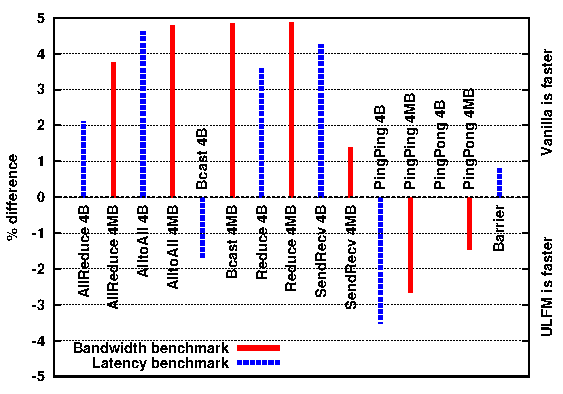
\includegraphics[width=.8\linewidth]{figures/IMB}
    \caption{Relative difference between \ulfm and Vanilla Open MPI on Shared Memory}
    \label{fig:ulfm:imb}
\end{figure}

The first set of tests demonstrates the overhead of the changes made in the \mpi 
implementation. This work builds on the work demonstrated in 
Chapter~\ref{chap:cof} to support \cof. The runtime found in \cof is the same for 
both versions of \mpi, so the performance discussions in 
Section~\ref{subsect:cof:performance:overhead} are also valid for \ulfm.

\subsubsection{Intel MPI Benchmarks}

We start with a demonstration of latency and bandwidth using the Intel MPI 
Benchmark test suite~\cite{IMB}. This suite has many tests to measure the 
performance of everything from collective operations to latency times. We run this 
test using ``Romulus'', a large shared memory machine at the University of 
Tennessee. In Figure~\ref{fig:ulfm:imb} we see that the impact of the \ulfm 
changes to \mpi are negligible, as expected. For tests where the default Open MPI 
performed better, the bar is above the center line, and for tests where \ulfm had 
better performance, the bar is below the center line. For all of the tests, the 
relative difference remains below 5\%, which is within the standard deviation of 
the tests on that machine, showing that any difference in the performance of the 
two implementations is negligible.

\begin{table}
	\captionof{table}{NetPIPE results on Smoky.}
	\label{tab:ulfm:netpipe}
	\begin{center}\sf\scriptsize
		\begin{tabular}{|l||r|r||r|r||r|}
			\multicolumn{6}{c}{1-byte Latency (microseconds) (cache hot)} \\
			\hline
			\cellcolor[gray]{0.7}\textbf{Interconnect}  & \cellcolor[gray]{0.7}\textbf{Vanilla}   & \cellcolor[gray]{0.7}\textbf{Std. Dev.} &
			\cellcolor[gray]{0.7}\textbf{Enabled}         & \cellcolor[gray]{0.7}\textbf{Std. Dev.} & \cellcolor[gray]{0.7}\textbf{Difference} \\
			\hline
			\cellcolor[gray]{0.9}Shared Memory &  0.8008 & 0.0093 &  0.8016 & 0.0161 &  0.0008 \\
			\cellcolor[gray]{0.9}TCP           & 10.2564 & 0.0946 & 10.2776 & 0.1065 &  0.0212 \\
			\cellcolor[gray]{0.9}OpenIB        &  4.9637 & 0.0018 &  4.9650 & 0.0022 &  0.0013 \\
			\hline
			\multicolumn{6}{c}{Bandwidth (Mbps) (cache hot)} \\
			\hline
			\cellcolor[gray]{0.7}\textbf{Interconnect}  & \cellcolor[gray]{0.7}\textbf{Vanilla}   & \cellcolor[gray]{0.7}\textbf{Std. Dev.} &
			\cellcolor[gray]{0.7}\textbf{Enabled}         & \cellcolor[gray]{0.7}\textbf{Std. Dev.} & \cellcolor[gray]{0.7}\textbf{Difference} \\
			\hline
			\cellcolor[gray]{0.9}Shared Memory &  10,625.92 &  23.46 &  10,602.68 & 30.73 & -23.24 \\
			\cellcolor[gray]{0.9}TCP           &   6,311.38 &  14.42 &   6,302.75 & 10.72 &  -8.63 \\
			\cellcolor[gray]{0.9}OpenIB        &   9,688.85 &   3.29 &   9,689.13 &  3.77 &   0.28 \\
			\hline
		\end{tabular}
	\end{center}
\end{table}

\subsubsection{NetPIPE}

The next test found in Table~\ref{tab:ulfm:netpipe} uses the NetPIPE~\cite{netpipe} 
benchmark (version 3.7) to measure the 1-byte latency and bandwidth of both 
Vanilla Open MPI and \ulfm. Here again, we find that any difference between the 
two implementations is within both the noise limit of the network and the standard 
deviation of the test, showing that the impact of the \ulfm modifications on a 
failure-free \mpi environment is minimal.

\begin{figure}[t]
    \centering
    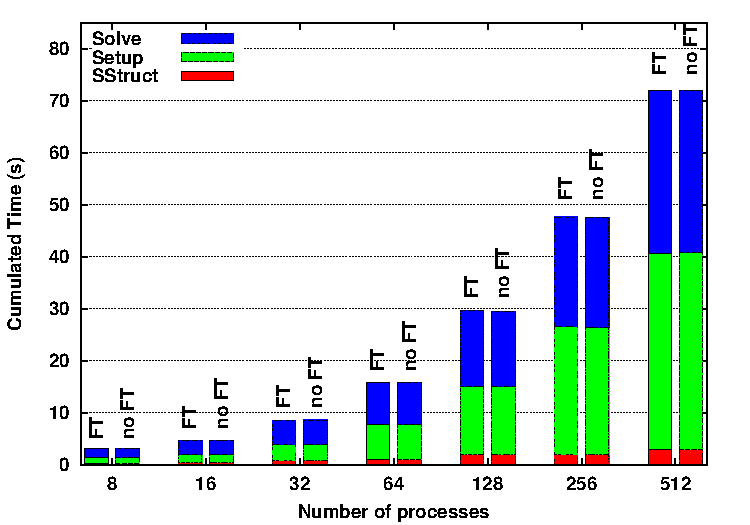
\includegraphics[width=.8\linewidth]{figures/bargraph}
    \caption{Comparison of Sequoia-AMG running at different scales with \ulfm and Vanilla Open MPI}
    \label{fig:ulfm:sequoia}
\end{figure}

\subsubsection{Sequoia-AMG}

To demonstrate the impact of the \ulfm modifications on a full application, we 
used the Sequoia-AMG~\cite{sequoiaAMG} benchmark on ``Smoky'', a 512 node cluster at Oak 
Ridge National Laboratory where each node contains four quad-core 2.0 GHz AMD 
Opteron processors with 2 GB of memory per core. The benchmark is an Algebraic 
Multi-Grid (AMG) linear system solver for unstructured mesh physics and makes 
heavy use of \mpi. We measured the weak scaling results and found that there was 
virtually no difference between the \ulfm MPI performance and the Vanilla Open MPI 
performance. It is important to remember the difference between the type of 
results we see here and the results seen in 
Section~\ref{subsec:ulfm:performance:qr}. These tests do not contain modifications 
to undergo failure or process recovery, but are only measuring the overhead of the 
\mpi implementation.

\subsection{\abft-QR Factorization}
\label{subsec:ulfm:performance:qr}

\begin{figure}[t]
    \centering
    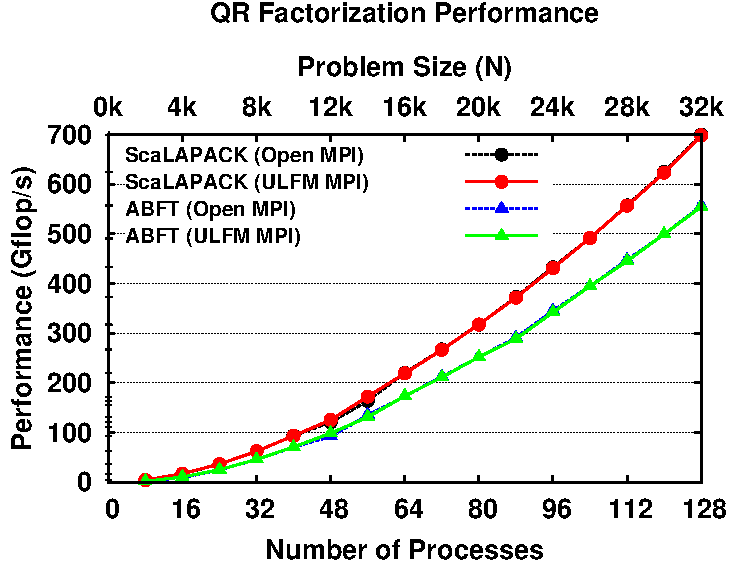
\includegraphics[width=\linewidth]{figures/g5k_results_weak}
    \caption{Weak-Scaling performance of ABFT-QR on Grid5000 'Graphene' compared to ScaLAPACK in both Vanilla Open MPI and the ULFM version}
    \label{fig:ulfm:qr-weak}
\end{figure}

\begin{figure}[t]
    \centering
    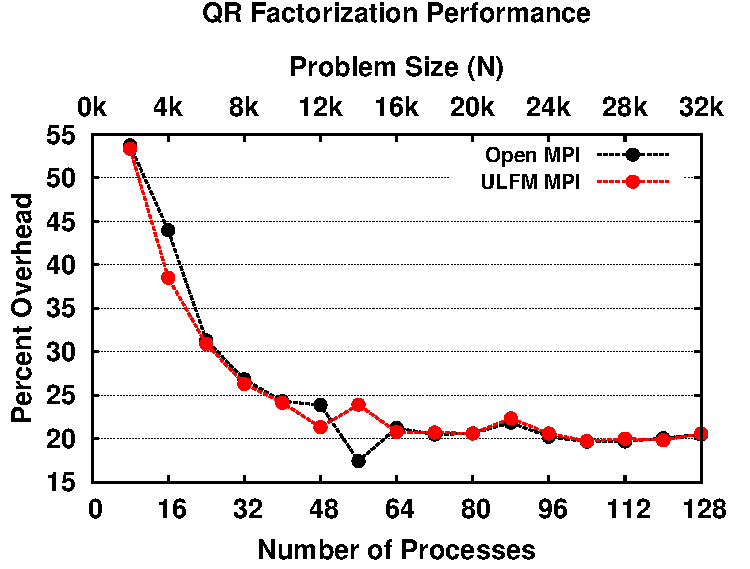
\includegraphics[width=\linewidth]{figures/g5k_results_weak_proportional}
    \caption{Overhead of ABFT with Vanilla Open MPI and ULFM MPI}
    \label{fig:ulfm:weak-overhead}
\end{figure}

\begin{figure}[t]
    \centering
    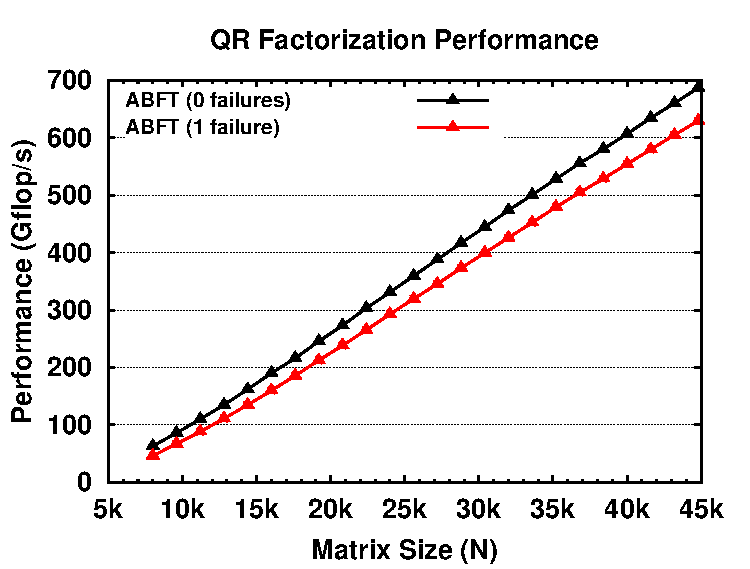
\includegraphics[width=\linewidth]{figures/g5k_results_flops}
    \caption{Strong-Scaling performance of ABFT-QR on Grid5000 'Graphene' with no failures and one failure}
    \label{fig:ulfm:qr-failure}
\end{figure}

\begin{figure}[t]
    \centering
    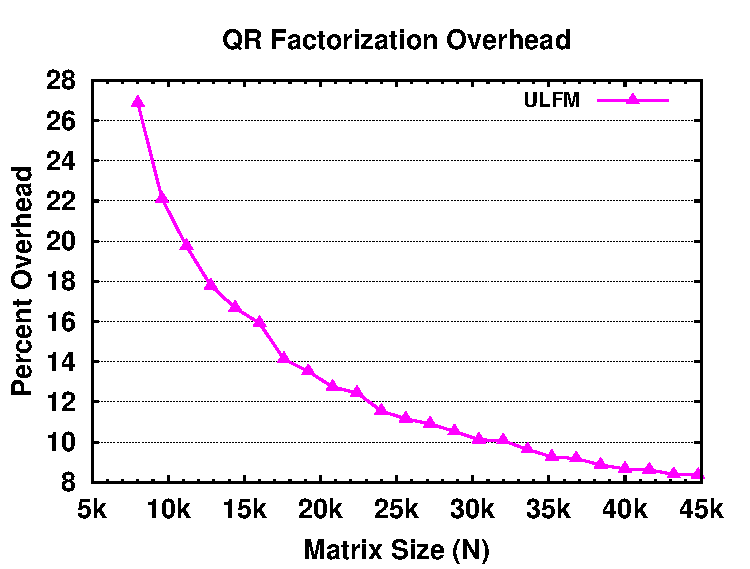
\includegraphics[width=\linewidth]{figures/g5k_results_proportional}
    \caption{Overhead of one failure with ABFT-QR on ULFM MPI}
    \label{fig:ulfm:failure-overhead}
\end{figure}

\begin{figure}[t]
    \centering
    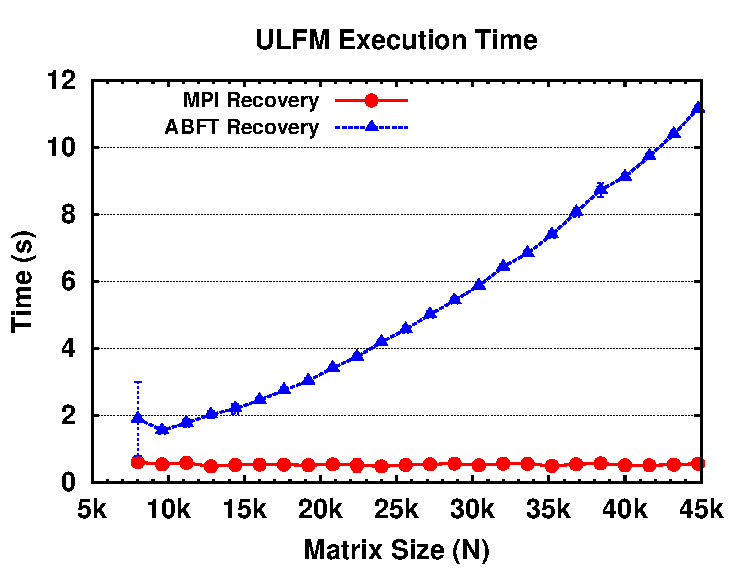
\includegraphics[width=\linewidth]{figures/g5k_results_ulfm}
    \caption{Recovery time of MPI and Data (via ABFT) on Grid5000}
    \label{fig:ulfm:qr-recovery}
\end{figure}

As discussed in Section~\ref{subsec:ulfm:apps:qr}, the \abft-QR Factorization code 
has been modified to work with \ulfm to demonstrate how \ulfm can be leveraged to 
provide fault tolerance to a ``real world'' algorithm. Here we discuss the 
performance of the algorithm using a machine found in 
Grid'5000~\footnote{ Acknowledgment: Experiments presented in this paper were 
carried out using the Grid'5000 experimental testbed, being developed under the 
INRIA ALADDIN development action with support from CNRS, RENATER and several 
Universities as well as other funding bodies (see https://www.grid5000.fr).}. We 
used the ``Graphene'' cluster at the Nancy site. ``Graphene'' is a 144 node 
cluster using Intel Xeon X3440 2.53 Ghz 4 core processors, 16 GB of memory, and 
Infiniband-20G cards. As with the IMB tests above, for all tests performed here, 
we used the \textit{tcp} BTL.

The first test in Figure~\ref{fig:ulfm:qr-weak} demonstrates the performance overhead 
of our modifications to the \ulfm library. In this graph, we see that our changes have 
almost no impact on the results of the test which we will use as an established fact 
for the remainder of the discussion. This test also demonstrates the weak scaling 
capability of the ABFT algorithm using both the original Open MPI library and the \ulfm 
MPI library. 

In Figure~\ref{fig:ulfm:weak-overhead}, we show the overhead of the \abft 
algorithm itself using the same original data. While the gap appears to grow in 
Figure~\ref{fig:ulfm:qr-weak}, Figure~\ref{fig:ulfm:weak-overhead} shows that the 
relative difference between the two implementations 
actually stabilizes. This is the expected result for this type of test. For small 
problem sizes, the overhead will be high because the problem is not large enough to 
fill the pipeline of the machines. However, as the problem size increases, the 
experienced overhead stabilizes at around 20\% of the execution time. While we expect 
that through more optimization, this overhead could shrink, perhaps significantly, it 
will never disappear entirely as the \abft algorithm will always incur overhead from 
the data protection schemes.

Now that the overhead of the \mpi implementation itself and the \abft code has been 
established, the most interesting result of the QR factorization test is to demonstrate 
the overhead of the failures themselves. To show this, we used a strong scaling test, 
where the number of processes is held steady at 128 nodes and the problem size 
increases from 8,000 to 44,000. The results of this test are not directly comparable to 
the results of the previous tests as the configuration of the \mpi library was slightly 
altered. Figure~\ref{fig:ulfm:qr-failure} demonstrates the performance of the \abft 
algorithm with no failures and again with one failure using our \ulfm implementation of 
\mpi. Here we see that the relative overhead of the failure seems to be relatively low 
and the algorithm still achieves good performance.

We quantify this overhead in Figure~\ref{fig:ulfm:failure-overhead} where we see that 
the overhead of the failure diminishes quickly to close to 8\%, though it would 
probably continue to drop at larger scales. We expect this value to decrease due to the 
relatively low overhead of failure recovery. The cost of recovery itself (as opposed to 
the data protection built into the \abft algorithm) is only the cost of replacing the 
failed process and repairing the data in the matrix. These costs are detailed in 
Figure~\ref{fig:ulfm:qr-recovery}. The \mpi recovery time stays constant as the matrix 
size increases and the number of processes remains constant. This number stays 
relatively low at around 400 milliseconds to perform all of the recovery 
operations (\mpifunc{REVOKE}, \mpifunc{SHRINK}, \mpifunc{SPAWN}, \mpifunc{MERGE}, 
and \mpifunc{SPLIT}). The \abft recovery time continues to scale with the problem 
size as the data recovery operations perform reductions across the entire matrix 
to calculate the missing data. Again these numbers are around the expected values 
and account for the disparity between the failure-free execution and the execution 
where a failure is injected early in the computation.

\section{Evaluation of \ulfm}

Where \cof fell short of many of the goals in Chapter~\ref{chap:goals}, \ulfm is 
purposely designed to fulfill each of them. It provides the maximum amount of 
\textbf{flexibility} for fault tolerance because it is a minimal set of functions which 
provide a platform on which other types of fault tolerance can be constructed. It 
maintains \textbf{resilience} in the face of failures by ensuring that the library 
provides sufficient failure notification to prevent deadlock and introduces new 
constructs to allow the application or library to introduce more consistency when 
necessary. While \textbf{productivity} is not the strength of \ulfm itself, it 
encourages new, portable libraries which will make the ideas of \ulfm more available to 
non-experts who are not as familiar with the theory of fault tolerance. More 
information about this can be found in Chapter~\ref{chap:apps}.

    \chapter{Fault Tolerant Applications and Libraries}
\label{chap:apps}

During the \ulfm design process, the specific intention has been to not promote 
one form of fault tolerance over another. The primary reason for this is because, to 
this point, no type of fault tolerance has emerged as a single solution to all 
applications and this situation is not expected to change in the future. Applications 
will always need to evaluate their execution method and choose the type of fault 
tolerance which best fits.

To this end, \ulfm was designed to support all types of fault tolerance by 
providing a high-performing, portable interface. One of the biggest barriers to 
entry in the current field of fault tolerance is the lack of portability for 
fault tolerant solutions, specifically those which involve MPI. No MPI 
implementation has become a de facto standard for fault tolerance and therefore 
none has not been adopted into the MPI Standard itself. It is our hope that this work 
will eventually provide that foundation upon with other solutions can build. While 
\ulfm can be a fault tolerance solution for some applications, the end goal of 
this work is to encourage other developers to create libraries which implement 
both established and new types of fault tolerance using the mechanisms provided.

This section will explore how fault tolerance can be implemented with \ulfm, both from an application perspective, and how libraries could be constructed using the constructs provided.

\section{Types of Fault Tolerance}
\label{sec:apps:types}

First we will evaluate the fault tolerance methods currently used in the research 
community and how they can be re-implemented using \ulfm as the foundation for 
the MPI communication.

\subsection{Automatic Methods}
\label{subsec:apps:types:auto}

Despite the development of new forms of recovery with the potential to 
replace it, checkpoint/restart has remained a staple of fault tolerance. This is 
primarily due to the fact that it is already ubiquitous, and it is simple to 
understand and use. Because of all this, there is no reason to believe that the 
use of checkpoint/restart is likely to diminish in the near future.

\ulfm makes bringing synchronous checkpoint/restart into the MPI application 
simple. An example of this is \cof as discussed in Chapter~\ref{chap:cof}. \cof 
uses small checkpoints, but vastly improves the restart time because it does not 
require the application to re-enter the batch queue system. \ulfm improves this 
scenario even more as it no longer requires most of the processes in the 
application to even restart. Instead, the application can roll back any processes 
which need to recover data, repair any communication objects in use, and continue 
with the existing MPI infrastructure.

Asynchronous checkpointing can also be added to \ulfm as an external library. 
Message logging can be implemented by using existing PMPI (MPI standard profiling interface) hooks to capture 
messages as they are sent and received. To recover, a library can provide a 
function which simplifies the process of spawning replacement processes, 
replaying messages to the new processes using the locally logged messages, and 
continuing the normal execution.

To implement replication and migration with \ulfm, again, the library would use 
PMPI hooks to capture messages between processes. This time, rather than logging 
the content of messages, the library would redirect messages to the appropriate 
processes in the case where they have been moved from their original rank. When 
the application (or some separate failure detector) detects a failure (or 
imminent failure), it can checkpoint the application, move it to a new processor, 
and restart it on the remote machine.

\subsection{Algorithm Based Fault Tolerance}
\label{subsec:apps:types:abft}

While \abft describes a wide range of algorithms, \ulfm has been uniquely 
designed to support them. Many \abft algorithms do not require that all processes 
which begin an application remain running to completion. An example of such a 
class of applications is a Monte-Carlo master/worker application where a master, 
or group of master processes, divide and distribute work to a pool of worker 
processes. If a process in the worker pool fails, the worker does not need to be 
replaced. Only the work needs to be recovered, and it is given to another worker 
to complete in its place. For these types of applications, \ulfm can often 
support them directly by providing the simple tool, \mpifunc{MPI\_COMM\_AGREE}. 
When a master process detects a failure, it removes the process from its internal 
list of alive workers (possibly informing other masters if they exist) and 
continues without any other MPI recover. When the application is ready to 
complete, the group of workers can call \mpifunc{MPI\_COMM\_AGREE} to determine 
if all of the master processes agree that they are finished or need to perform 
some other recovery.

For applications which require all processes to continue running through the 
application's completion, \ulfm again provides all of the tools necessary. Upon 
failure, the application should call \mpifunc{MPI\_COMM\_REVOKE} to inform all 
other processes about the process failure, then the processes collectively call 
\mpifunc{MPI\_COMM\_SHRINK} to generate a working communicator without the 
failed processes. Next, the processes call the existing MPI function 
\mpifunc{MPI\_COMM\_SPAWN} to replace any failed processes with new ones. 
\mpifunc{MPI\_INTERCOMM\_MERGE} will create a more traditional intracommunicator 
from the intercommunicator generated by \mpifunc{MPI\_COMM\_SPAWN}. If the 
original ranks were important, the application can use 
\mpifunc{MPI\_COMM\_SPLIT} where all processes contribute the same color to 
signify that they will all remain in the same communicator and contribute their 
desired rank to the ``key'' value. At this point, the application is ready to 
repair any lost data and continue. These functions can be combined into a 
convenience function to simplify development, but the construction of an 
entirely new library is unnecessary for most forms of \abft.

\subsection{Transactional Fault Tolerance}
\label{subsec:apps:types:transactions}

Transactional fault tolerance is similar to the rollback recovery methods found 
in checkpoint/restart protocols. However, it also implies more automatic 
recovery than is provided in checkpoint/restart. Transactions can be constructed 
by adding a new mechanism to expand the functionality of
\mpifunc{MPI\_COMM\_AGREE}. In addition to the agreement algorithm, the new 
function can store the state of the running application when the agreement 
algorithm determines that no failures occurred in the previous transaction, or 
it can roll the application back to a known good state when the previous 
transaction fails. In addition to rolling the existing processes back to a 
previous state, the library can perform the recovery methods described in 
Section~\ref{subsec:apps:types:abft} to restore any failed ranks using the 
existing data from the previous transaction.

\subsection{Collective Consistency}
\label{subsec:apps:types:consistency}

One of the design decisions made when envisioning \ulfm was to have failure 
knowledge be local. Failure notification on one process is no guarantee that any 
other processes are also aware of the failure. This decision was reached for 
performance reasons, however some applications may be willing to pay this 
performance cost in exchange for global knowledge of failures. For these 
applications, a library can easily be constructed to 
include collective consistency using the tools provided in \ulfm. The goal of 
collective consistency is to ensure that all processes involved in a 
communication operation return an error code uniformly. To do this, a library 
can add a call to \mpifunc{MPI\_COMM\_AGREE} after the completion of each 
communication function which decides the status of previous operations. If any 
process returned a failure, then all remaining processes can agree on the return 
code and provide the same value upon exit. This allows the application to ignore 
the implications of local failure notification and perform recovery accordingly.

\section{Library Construction}
\label{sec:apps:library}

Given the emphasis laid on the ability to construct many varieties of fault 
tolerance using the tools provided by \ulfm, one of the most important 
demonstrations to be made should be properly constructing libraries. The 
technique to do so was not as immediately apparent as it may seem so we detail 
it here to simplify the process in the future. This is not the only technique to 
properly construct a fault tolerant library on top of \ulfm, but it can be used 
as a starting point for future work. More details, including a complete code example can be found in Appendix~\ref{appdx:library}.

\subsection{Initialization}
\label{subsec:apps:library:init}

As with many scientific libraries, before using a library built on \ulfm, it is 
advisable to create an initialization function. In addition to any usual data 
initialization which may occur during this time, this is also where any 
sub-communicators can be created. It is important to not base any communicators 
on \mpifunc{MPI\_COMM\_WORLD} as this communicator will become broken and out of 
date immediately following the first recovery or dynamic processing operation. Once a process has failed, there 
is no way to repair \mpifunc{MPI\_COMM\_WORLD} to its original state or to 
include any new processes which may be spawned to replace the failed processes. 
To solve this problem, applications should provide another communicator, possibly 
even a simple duplicate of \mpifunc{MPI\_COMM\_WORLD}, into the library through 
the initialization function so that sub-communicators can be constructed from 
this communicator, rather than \mpifunc{MPI\_COMM\_WORLD}, as has become a 
standard practice in many MPI libraries.

\subsection{Status Object}
\label{subsec:apps:library:status}

Though not required, a status object can greatly simplify recovery later in an 
application. The status object can store useful pieces of data to be passed back 
and forth around library functions, but for the purposes of fault tolerance, the 
status object keeps track of the status of the most recent function calls. When 
a function is called, the object is passed into the function and the 
status of the function is updated throughout its execution. If a failure occurs 
and data is being recovered, the library can refer to the status object to 
discover what kinds of data to recover and signal the function that the library 
has been repaired. A status object is stored in the space of the calling 
application or library rather than within the library itself. The reason for 
this is so the status object may remain easily savable for fault tolerance, either 
by checkpointing, storage on a remote node, or duplication. 

\subsection{The Three R's}

When a failure does occur, a fault tolerant library using \ulfm should perform 
``Three R's'' to get the library back into a functional state.

\subsubsection{Revoke}

First, the library should call \mpifunc{MPI\_COMM\_REVOKE} on all internal communicators 
to ensure that all other processes are alerted to the process failure. As most 
of the communicators will be reconstructed when the library is later being 
repaired anyway, this step does not introduce a level of overhead which would 
otherwise not have been present. Once all communicators have been revoked, it is 
safe to return from the library.

\subsubsection{Return}

The low level libraries should not attempt to perform process recovery 
automatically. The reason for this is that libraries generally do not make their 
internal communicators available to outside entities. If a library were to 
repair its own communicators by creating new processes to replace any failures, 
other libraries or parts of the application would no longer have access to these 
new processes as they would not be able to communicate through any existing 
channels. While it would be possible to create new communicators to solve this 
problem, the complexity introduced would not justify the effort and invalidate the 
convenience of performing the automatic recovery in the first place. In addition, 
the act of spawning new processes requires access to the original command line 
parameters. While these could be passed into the library to facilitate recovery, 
it is simpler to perform all of the actions at the same level, from the 
original application.

\subsubsection{Repair}

Once the libraries have revoked their internal communicators and returned to the 
highest level, the MPI recovery can begin. This should be a collaborative 
process between the application and all of the lower level libraries, however it 
should start with the application repairing MPI first. Depending on the 
application, this repair operation could include spawning new processes to 
replace any failures, or it could simply be calling \mpifunc{MPI\_COMM\_SHRINK} 
to remove any failed processes from the communicators. Once the application has 
repaired MPI, it should allow the libraries to repair themselves by providing 
the new MPI communicator to their repair functions. If the repair function will 
also repair any missing or corrupt data, the status object should also be 
included so the libraries will know the status of their previous operations and 
can recover accordingly. The libraries should continue to call any lower level 
repair functions for libraries on which they depend until all libraries have 
been appropriately repaired.

\begin{figure}
    \centering
    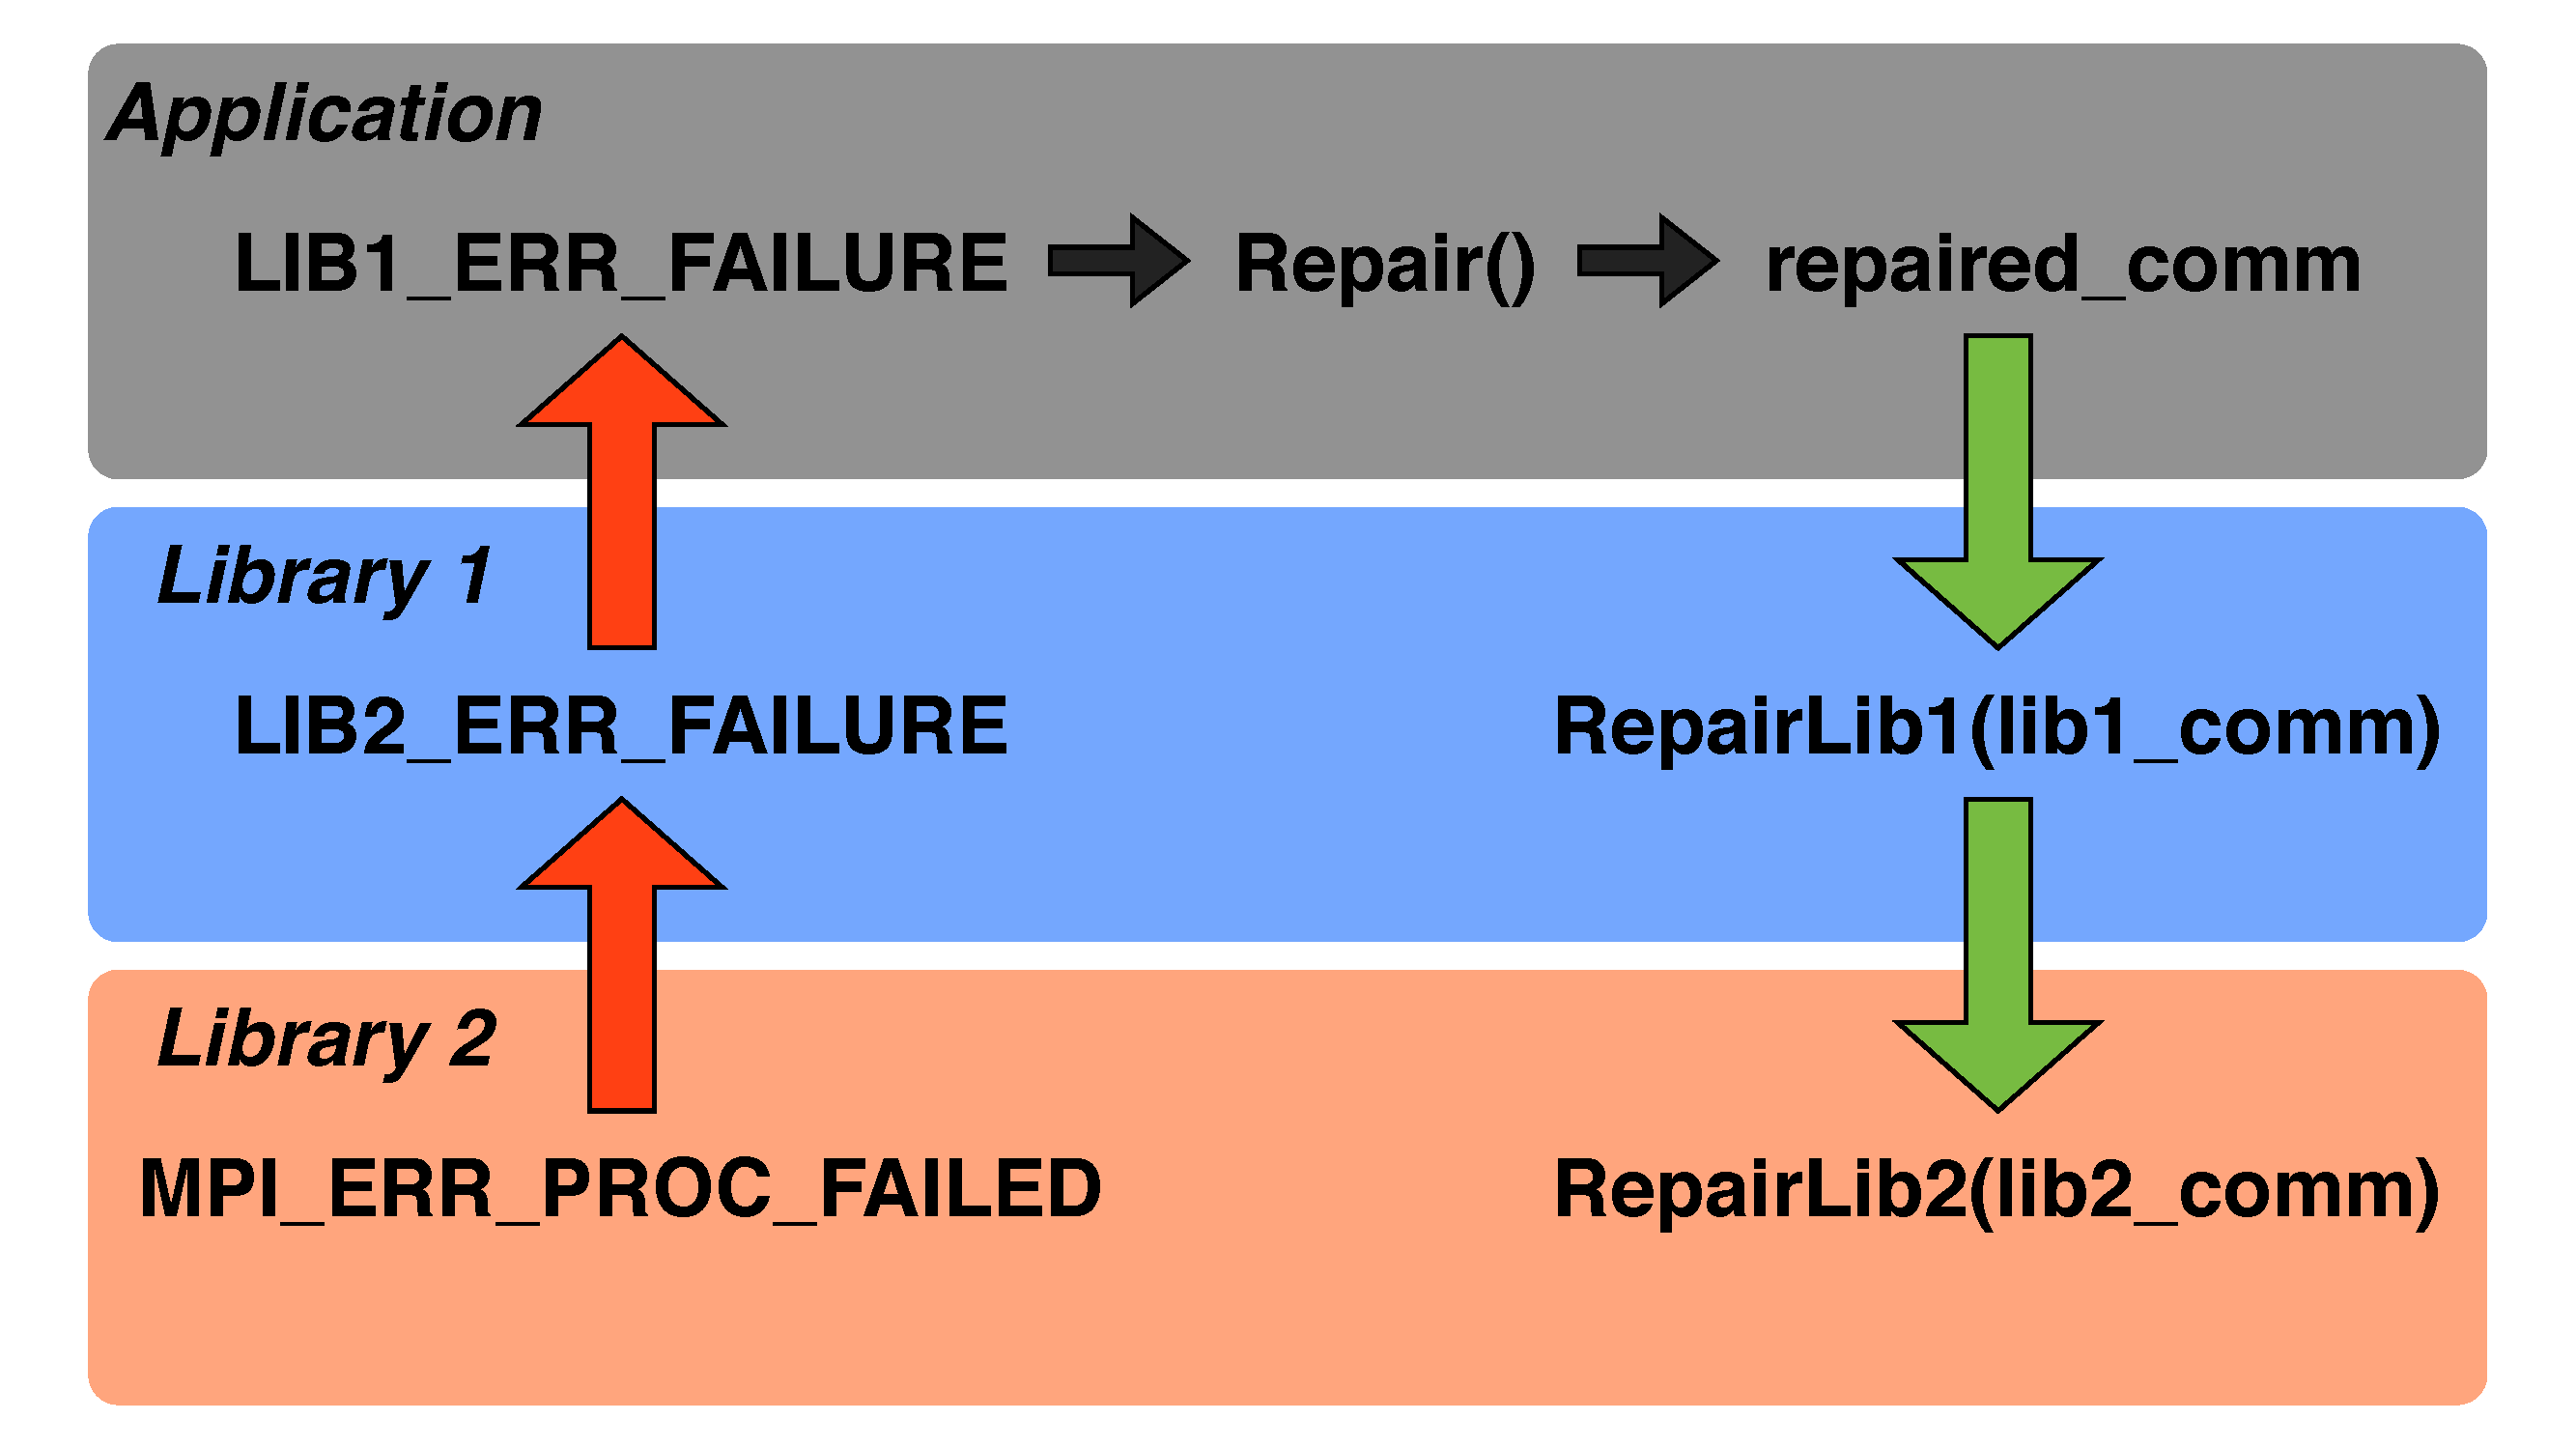
\includegraphics[width=\linewidth]{figures/libraries}
    \caption{ABFT QR and one \cof recovery on Kraken (Lustre).}    	\label{fig:apps:library-repair}	
\end{figure}

\subsubsection{Overview}

Figure~\ref{fig:apps:library-repair} demonstrates the hierarchy of libraries and 
how they should be repaired. Errors will most likely be detected by the lowest 
level library currently in use. The libraries should recursively revoke their 
communicators and return to the next level. The application should repair the 
MPI library using the appropriate measures and allow the libraries to do the same 
by calling their respective repair functions. Once all of the recovery is 
complete, the application can repeat its call to the last function it was 
attempting and execution can continue. 

Obviously, this pattern will not apply to all libraries. Some libraries 
developed to provide MPI fault tolerance directly may perform recovery 
themselves without returning to the MPI application. Some libraries may not 
include MPI calls which would necessitate recovery. However, this is a starting 
point for those interested in constructing fault tolerant MPI libraries. For a 
more complete example, see Appendix~\ref{appdx:library}.

    \chapter{Future Work and Conclusions}
\label{chap:conclusions}

\section{Summary}
\label{chap:conclusions:summary}

As machine sizes and problem runtimes have increased over the decades, the rise 
of fault tolerance as a field of study has increased to match. Early on, 
applications developed methods of error checking and recovery to prevent faults from 
causing inconsistent results. Later, as the 
types of machines on which applications were being run evolved from large 
mainframe types of machines to Networks of Workstations (NoWs), checkpointing 
became important. Because workstations were considered unreliable as they could 
quickly become unavailable due either local use, or more common failures due to 
cheaper hardware, applications needed to be able to save their state during 
execution and possibly migrate from one machine to another. This started as a 
transparent feature that automatically performed checkpointing and migration and 
transitioned into a sophisticated system which could be triggered on-demand by an 
application, even performing asynchronous checkpoints which could later be used, 
along with message logging, to roll back applications to previous states.

All of these methods of fault tolerance were sufficient for the machines on which 
they were designed to function. The scale of the machines did not cause 
contention for bandwidth to stable storage, and failures did not occur with enough 
frequency to eclipse the time needed to perform a checkpoint. In recent years and 
going forward to projected machine architectures in the near future, these 
statements will not remain true. Machine sizes have already eclipsed the million 
core mark and runtimes for such large scale, capability applications extend to 
multiple days. 

To solve this problem, new codes using Algorithm Based Fault Tolerance (\abft) 
are now being designed which can repair themselves with very little data 
necessary. These algorithms have been proven to be effective and 
numerically stable, but to continue their parallel execution, they require a 
Message Passing Interface (\mpi) library which can consistently provide 
communication channels, even after a process failure makes some subset of the 
machine unusable.

As a first step to provide the desired \mpi implementation, we developed a new 
protocol called Checkpoint-on-Failure (\cof). This protocol provides an 
opportunity for applications to save their state \textit{after} the application 
has detected a process failure. By changing the default MPI Error Handler from 
\mpifunc{MPI\_ERRORS\_ARE\_FATAL} to \mpifunc{MPI\_ERRORS\_RETURN} or another custom 
error handler, the application is alerted to process failures and can incur the 
overhead of saving state only when process failures actually occur, rather than 
periodically throughout the application execution. In Chapter~\ref{chap:cof}, we 
demonstrated the low overhead and recovery time that \cof provides.

Once the foundational work, such as a resilient runtime, was completed in the 
\cof implementation, we introduced a more ambitious project. User Level Failure 
Mitigation (\ulfm), is a new chapter for the \mpi Standard which provides a 
complete solution for fault tolerance, not just an improved checkpoint/restart 
protocol. \ulfm allows \abft codes to continue execution on all non-failed 
processes and replace failed processes with new ones which can be joined with 
already existing processes using (already standardized) MPI-2 dynamic processing 
functions. It does this by providing a minimal interface which includes failure 
detection, failure notification, and deadlock resolution mechanisms, while 
encouraging the development of new libraries to envision more complex recovery 
mechanisms, such as transactions, collective consistency, or automatic recovery.

\section{Future Work}
\label{chap:conclusions:future}

The tools developed in this work are extensive and sufficient for many styles of 
fault tolerance. However, they are not simple enough for developers not 
familiar with fault tolerance methods to construct complex recovery mechanisms. 
For this work to continue to be successful, more libraries will need to follow to 
provide interfaces which make fault tolerance more accessible.

One of the greatest challenges currently faced by researchers in the field of 
fault tolerance is apathy from those who they attempt to convince to adopt new fault 
tolerance techniques. For many years, scientists who develop codes for high 
performance architectures have been warned about the impending need for fault 
tolerance and the requirement that their codes be refactored to implement new 
protocols. However, the problems were largely resolved by implementing new 
automatic fault tolerance solutions, such as checkpoint/restart, which did not 
require that existing codes be modified, only that they be recompiled to include 
a new library.

Now, as new projections demonstrate the need for new methods of fault tolerance 
rather than an improved automatic solution~\cite{BosilcaINRIARep7950}, the need is not to 
convince developers to refactor their existing scientific codes to include fault 
tolerance, but to first convince researchers to develop easy to use, portable 
libraries which simplify the process of including fault tolerance in existing 
codes and provide resilience options for new codes being developed. These 
libraries will be much more adoptable and will speed the inclusion of fault 
tolerance in codes which already have expressed a need for such tools.

    
    %%%%%%%%%%%%%%%%%%%%%%%%%%%%%%%%%%%%%%%%%%%%%%%%%%%%%%%%%%%%%%%%%%%%%%%%%%%%%%%%%%%%%%%%%%%%%%%%%%%%%
    % BIBLIOGRAPHY
    %%%%%%%%%%%%%%%%%%%%%%%%%%%%%%%%%%%%%%%%%%%%%%%%%%%%%%%%%%%%%%%%%%%%%%%%%%%%%%%%%%%%%%%%%%%%%%%%%%%%%
    \makeBibliographyPage % make the bibliography title page - can be edited in ut-thesis-template.tex
    \bibliographystyle{IEEEtranS} % bibliography style - recommend using apalike-doi as it hyperlinks DOIs
    \bibliography{phd-dissertation} % references.bib included in the references directory
    
    %%%%%%%%%%%%%%%%%%%%%%%%%%%%%%%%%%%%%%%%%%%%%%%%%%%%%%%%%%%%%%%%%%%%%%%%%%%%%%%%%%%%%%%%%%%%%%%%%%%%%
    % APPENDIX - OPTIONAL - COMMENT IF NOT NEEDED
    %%%%%%%%%%%%%%%%%%%%%%%%%%%%%%%%%%%%%%%%%%%%%%%%%%%%%%%%%%%%%%%%%%%%%%%%%%%%%%%%%%%%%%%%%%%%%%%%%%%%%
    \appendixpage
    \appendix
    %
% Ticket 323
% https://svn.mpi-forum.org/trac/mpi-forum-web/ticket/323
%
% Based on the wiki page
% https://svn.mpi-forum.org/trac/mpi-forum-web/wiki/User_Level_Failure_Mitigation
%
%%%%%%%%%%%%%%%%%%%%%%%%%%%%%%%%%%%%%%%%%%%%%%%%%%%%%%%%%%%%%%%%%%%%%%

\renewcommand*\descriptionlabel[1]{\hspace\labelsep\it #1}

\appendixchapter{Process Fault Tolerance}
\label{chap:ft}
\subsubsection*{Chapter Submitted to MPI Forum. Section references not preceded by an \texttt{A} refer to the MPI 3.0 Standard document.}

\appendixsection{Introduction}
\label{sec:ft-intro}

Long running and large scale applications are at increased risk of encountering
process failures during normal execution. We consider a
process failure as a fail-stop failure; failed processes become permanently
unresponsive to communications.  This chapter introduces the \mpi features
that support the development of applications and libraries that can tolerate
process failures.  The approach described in this chapter is intended to prevent
the deadlock of processes while avoiding impact on the failure-free execution of
an application.

The expected behavior of \mpi in the case of a process failure is defined
by the following statements: any \mpi operation that involves a failed process
must not block indefinitely, but either succeed or raise an \mpi exception (see
Section~\ref{sec:ft-notification}); an \mpi operation that does not involve the
failed process will complete normally, unless interrupted by the user through
provided functionality. Asynchronous failure propagation is not required. If an
application needs global knowledge of failures, it can use the interfaces
defined in Section~\ref{sec:ft-functions} to explicitly propagate locally
detected failures.  

An implementation that does not tolerate process failures must provide the
interfaces and semantics defined in this chapter as long as no failure 
occurred. It must never raise an exception of class 
\mpifunc{MPI\_ERR\_PROC\_FAILED} or \mpifunc{MPI\_ERR\_PENDING}
because of a process failure.
This chapter does not define process failure semantics for the operations
specified in Chapters 10, 11 and 12, therefore they remain undefined by the \mpi standard.

\begin{description}

\item[Advice to Users] {Many of the operations and semantics described in
this chapter are only applicable when the \mpi application has replaced
the default error handler \mpifunc{MPI\_ERRORS\_ARE\_FATAL} on, at least,
\mpifunc{MPI\_COMM\_WORLD}.}

\end{description}

\appendixsection{Failure Notification}
\label{sec:ft-notification}

This section specifies the behavior of an \mpi communication
operation when
failures occur on processes involved in the communication. A process is
considered involved in a communication if any of the following is true:

\begin{enumerate}

    \item the operation is collective and the process appears in one of the
        groups {of the associated communication object};

    \item the process is a specified or matched destination or source in a
        point-to-point communication;

	\item the operation is an \mpifunc{MPI\_ANY\_SOURCE} receive operation and the
        failed process belongs to the source group.

\end{enumerate}


Therefore, if an operation does not involve a failed process (such as a point-to-point 
message between two non-failed processes), it must not raise a process
failure exception. 

\begin{description}

\item[Advice to Implementors] {A correct \mpi implementation may provide
failure detection only for processes involved in an ongoing operation,
and postpone detection of other failures until necessary.  Moreover, as
long as an implementation can complete operations, it may choose to
delay raising an error. Another valid implementation might choose to
raise an error as quickly as possible.}

\end{description}


Non-blocking operations must not raise an exception about process failures during
initiation. All process failure errors are postponed until the corresponding
completion function is called.

\appendixsubsection{Startup and Finalize}
\label{sec:ft-notification:init-finalize}

\begin{description}

\item[Advice to Implementors] {If a process fails during
\mpifunc{MPI\_INIT} but its peers are able to complete the \mpifunc{MPI\_INIT} 
successfully, then a high quality implementation will 
return \mpifunc{MPI\_SUCCESS} and delay the reporting of the process failure 
to a subsequent \mpi operation.}

\end{description}

\mpifunc{MPI\_FINALIZE} will complete successfully even in the presence of process failures.


\begin{description}

\item[Advice to Users] {Considering Example 8.7 in Section 8.7, 
the process with rank 0 in \mpifunc{MPI\_COMM\_WORLD} may have failed before, 
during, or after the call to \mpifunc{MPI\_FINALIZE}.
\mpi only provides failure detection capabilities up to when 
\mpifunc{MPI\_FINALIZE} is invoked and provides no support for fault tolerance 
during or after \mpifunc{MPI\_FINALIZE}. Applications are encouraged to implement 
all rank-specific code before the call to \mpifunc{MPI\_FINALIZE} 
to handle the case where process 0 in \mpifunc{MPI\_COMM\_WORLD} fails.}

\end{description}

\appendixsubsection{Point-to-Point and Collective Communication}
\label{sec:ft-notification:p2p-coll-comm}

An \mpi implementation raises the following error classes to notify
users that a point-to-point communication operation could not complete
successfully because of the failure of involved processes:

\begin{itemize}

\item \mpifunc{MPI\_ERR\_PENDING} indicates, for a non-blocking communication,
   that the communication is a receive operation from 
   \mpifunc{MPI\_ANY\_SOURCE} and no matching send has been posted, yet 
    a potential sender process has failed. Neither the operation nor 
    the request identifying the operation are completed. Note that the
    same error class is also used in status when another communication
    raises an exception during the same operation (as defined in 
    Section 3.7.5).
	
\item In all other cases, the operation raises an exception of class
    \mpifunc{MPI\_ERR\_PROC\_FAILED} to indicate that the failure prevents the
    operation from following its failure-free specification. If there is a
    request identifying the point-to-point communication, it is completed.
    Future point-to-point communication with the same process on this 
    communicator must also raise \mpifunc{MPI\_ERR\_PROC\_FAILED}.

\end{itemize}

\begin{description}

\item[Advice to Users] {To acknowledge a failure and discover which processes failed, the user should
call \mpifunc{MPI\_COMM\_FAILURE\_ACK} (as defined in
Section~\ref{sec:ft-functions:commfunctions}).}

\end{description}

When a collective operation cannot be completed because of the failure of
an involved process, the collective operation raises an error of class 
\mpifunc{MPI\_ERR\_PROC\_FAILED}. 

\begin{description} 

\item[Advice to Users] {Depending on how the collective operation is implemented and when a process
failure occurs, some participating alive processes may raise an exception while
other processes return successfully from the same collective operation. For
example, in \mpifunc{MPI\_BCAST}, the root process may succeed before a failed
process disrupts the operation, resulting in some other processes raising an
error. 
%
However, it is noteworthy that for collective operations on an intracommunicator
in which all processes contribute to the result and all
processes receive the result, processes which do not enter the
operation due to process failure provoke all surviving ranks to raise
\mpifunc{MPI\_ERR\_PROC\_FAILED}. 
%
Similarly, for the same collective
operations on an intercommunicator, a process in the remote group which failed
before entering the operation has the same effect on all surviving ranks of the
local group.}

\item[Advice to Users] {Note that communicator creation functions (like \mpifunc{MPI\_COMM\_DUP} or
\mpifunc{MPI\_COMM\_SPLIT}) are collective operations. As such, if a failure
happened during the call, an error might be raised at some processes while
others succeed and obtain a new communicator.  While it is valid to communicate
between processes which succeeded to create the new communicator, it is the
responsibility of the user to ensure that all involved processes have a
consistent view of the communicator creation, if needed.
%
A conservative solution is to have each process either revoke 
(see Section~\ref{sec:ft-functions:commfunctions}) the parent communicator if the
operation fails, or call an \mpifunc{MPI\_BARRIER} on the parent communicator
and then revoke the new communicator if the \mpifunc{MPI\_BARRIER} fails.}

\end{description}

When a communication operation raises an exception related to process failure, the
content of the output buffers is \emph{undefined}.

\appendixsubsection{Dynamic Process Management}
\label{sec:ft-notification:dyn-process}


Dynamic process management functions require some additional semantics from the
\mpi implementation as detailed below.

\begin{enumerate}

    \item If the \mpi implementation raises an error related to process
        failure to the root process of \mpifunc{MPI\_COMM\_CONNECT} or
        \mpifunc{MPI\_COMM\_ACCEPT}, at least the root processes of both
        intracommunicators must raise the same error of class
        \mpifunc{MPI\_ERR\_PROC\_FAILED} (unless required to raise
        \mpifunc{MPI\_ERR\_REVOKED} as defined by~\ref{sec:ft-functions:commfunctions}).

    \item If the \mpi implementation raises an error related to
        process failure to the root process of \mpifunc{MPI\_COMM\_SPAWN}, no spawned
        processes should be able to communicate on the created
        intercommunicator.

\end{enumerate}

\begin{description}

\item[Advice to Users] {As with communicator creation functions, it is
possible that if a failure happens during dynamic process management
operations, an error might be raised at some processes while others succeed
and obtain a new communicator.}

\end{description}

\appendixsubsection{One-Sided Communication}
\label{sec:ft-notification:one-sided}


As with all nonblocking operations, one-sided communication operations should
delay all failure notification until their synchronization operations which may raise
\mpifunc{MPI\_ERR\_PROC\_FAILED} (see Section~\ref{sec:ft-notification}). If the
implementation raises an error related to process failure from the
synchronization function, the epoch behavior is unchanged from the definitions
in Section 11.4. As with collective operations over \mpi communicators, it is
possible that some processes have detected a failure and raised
\mpifunc{MPI\_ERR\_PROC\_FAILED}, while others returned \mpifunc{MPI\_SUCCESS}. 


Unless specified below, the state of memory
targeted by any process in an epoch in which operations raised an error
related to process failure is undefined.

\begin{enumerate}

    \item If a failure is to be reported during active target communication
        functions \mpifunc{MPI\_WIN\_COMPLETE} or \mpifunc{MPI\_WIN\_WAIT} (or the non-blocking
        equivalent \mpifunc{MPI\_WIN\_TEST}), the epoch is considered completed and all
        operations not involving the failed processes must complete
        successfully.

    \item If the target rank has failed, \mpifunc{MPI\_WIN\_LOCK} and \mpifunc{MPI\_WIN\_UNLOCK} 
    	operations raise an error of class \mpifunc{MPI\_ERR\_PROC\_FAILED}.
        %
        If the owner of a lock has failed, the lock cannot be acquired again,
        and all subsequent operations on the lock must raise \mpifunc{MPI\_ERR\_PROC\_FAILED}.

\end{enumerate}

\begin{description}

\item[Advice to Users] {It is possible that request-based RMA operations
complete successfully while the enclosing epoch completes by raising error due
to process failure.  In this scenario, the local buffer is valid but the
remote targeted memory is undefined.}

\end{description}

\appendixsubsection{I/O}
\label{sec:ft-notification:io}

I/O error classes and their consequences are defined in
Section 13.7. The following section
defines the behavior of I/O operations when MPI process failures prevent their
successful completion.
%
Since collective I/O operations may not synchronize with other processes,
process failures may not be reported during a collective I/O operation. If a
process failure prevents a file operation from completing, an \mpi exception of
class \mpifunc{MPI\_ERR\_PROC\_FAILED} is raised.
%
Once an \mpi implementation has raised an error of class
\mpifunc{MPI\_ERR\_PROC\_FAILED}, the state of the file pointer is
\emph{undefined}.

\begin{description}
    
\item[Advice to Users]{Users are encouraged to use \mpifunc{MPI\_COMM\_AGREE} on a communicator
containing the same group as the file handle, to deduce the completion status of
collective operations on file handles and maintain a consistent view of file
pointers.}

\end{description}

\appendixsection{Failure Mitigation Functions}
\label{sec:ft-functions}

\appendixsubsection{Communicator Functions}
\label{sec:ft-functions:commfunctions}

 \mpi provides no guarantee of global knowledge of a process failure. Only
processes involved in a communication operation with the failed process are
guaranteed to eventually detect its failure (see
Section~\ref{sec:ft-notification}). If global knowledge is required, \mpi
provides a function to revoke a communicator at
all members.

\subsubsection*{MPI\_COMM\_REVOKE( comm ) \\
\begin{tabular*}{1.0\textwidth}{@{\extracolsep{\fill}} l l c r }
  \texttt{IN} & \texttt{comm} & & communicator (handle) \\
\end{tabular*}}

This function notifies all processes in the groups (local and remote) associated
with the communicator \textit{comm} that this communicator is now considered
revoked. This function is not collective and therefore does not have a matching 
call on remote processes. It is erroneous to call
\mpifunc{MPI\_COMM\_REVOKE} on a communicator for which no operation raised an
\mpi exception related to process failure. All alive processes belonging to
\textit{comm} will be notified of the revocation despite failures. 
The revocation of a communicator completes any non-local \mpi operations on
\textit{comm} by raising an error of class \mpifunc{MPI\_ERR\_REVOKED},
with the exception of \mpifunc{MPI\_COMM\_SHRINK} and
\mpifunc{MPI\_COMM\_AGREE} (and its nonblocking equivalent). A communicator
becomes revoked as soon as:

\begin{enumerate} 
    
    \item
        \mpifunc{MPI\_COMM\_REVOKE} is locally called on it;
    
    \item Any \mpi operation raised an error of class \mpifunc{MPI\_ERR\_REVOKED}
        because another process in \textit{comm} has called \mpifunc{MPI\_COMM\_REVOKE}.
            
\end{enumerate}


Once a communicator has been revoked, all subsequent non-local operations on that
communicator, with the exception of \mpifunc{MPI\_COMM\_SHRINK} and \mpifunc{MPI\_COMM\_AGREE}
(and its nonblocking equivalent), are considered local and must
complete by raising an error of class \mpifunc{MPI\_ERR\_REVOKED}. 

\begin{description}

\item[Advice to Users] {High quality implementations are encouraged to do their best to free resources locally when the user calls free operations on revoked communication objects, or communication objects containing failed processes.}

\end{description}

\subsubsection*{MPI\_COMM\_SHRINK( comm, newcomm ) \\
\begin{tabular*}{1.0\textwidth}{@{\extracolsep{\fill}} l l c r }
  \texttt{IN} & \texttt{comm} & & communicator (handle) \\
  \texttt{OUT} & \texttt{newcomm} & & communicator (handle) \\
\end{tabular*}}

This collective operation creates a new intra or inter communicator \textit{newcomm} from
the revoked intra or inter communicator \textit{comm} respectively by
excluding its failed processes as detailed below.  It is erroneous \mpi code to
call \mpifunc{MPI\_COMM\_SHRINK} on a communicator which has not been
revoked (as defined above) and will raise an error of class \mpifunc{MPI\_ERR\_ARG}. 


%
This function must not raise an error due to process failures (error classes
\mpifunc{MPI\_ERR\_PROC\_FAILED} and \mpifunc{MPI\_ERR\_REVOKED}).  All
processes that succeeded agreed on the content of the group of processes that
failed.  This group includes at least every process failure that has raised an
\mpi exception of class \mpifunc{MPI\_ERR\_PROC\_FAILED} or
\mpifunc{MPI\_ERR\_PENDING}.  The call is semantically equivalent to an
\mpifunc{MPI\_COMM\_SPLIT} operation that would succeed despite failures, and
where living processes participate with the same color, and a key equal to their
rank in \textit{comm} and failed processes implicitly contribute
\mpifunc{MPI\_UNDEFINED}. 

\begin{description}

\item[Advice to Users] {This call does not guarantee that all processes in
\textit{newcomm} are alive.  Any new failure will be detected in
subsequent \mpi operations.}

\end{description}

\subsubsection*{MPI\_COMM\_FAILURE\_ACK( comm ) \\
\begin{tabular*}{1.0\textwidth}{@{\extracolsep{\fill}} l l c r }
  \texttt{IN} & \texttt{comm} & & communicator (handle) \\
\end{tabular*}}

This local operation gives the users a way to \emph{acknowledge} all locally notified
failures on \textit{comm}. After the call, unmatched \mpifunc{MPI\_ANY\_SOURCE} receptions
that would have raised an error code \mpifunc{MPI\_ERR\_PENDING} due to process failure (see
Section~\ref{sec:ft-notification:p2p-coll-comm}) proceed without further reporting
of errors due to those acknowledged failures.

\begin{description}

\item[Advice to Users] {Calling \mpifunc{MPI\_COMM\_FAILURE\_ACK} on a communicator
with failed processes does not allow that communicator to be used
successfully for collective operations.  Collective communication on a
communicator with acknowledged failures will continue to raise an error
of class \mpifunc{MPI\_ERR\_PROC\_FAILED} as defined in
Section~\ref{sec:ft-notification:p2p-coll-comm}. To reliably use collective
operations on a communicator with failed processes, the communicator
should first be revoked using \mpifunc{MPI\_COMM\_REVOKE} and then a new
communicator should be created using \mpifunc{MPI\_COMM\_SHRINK}.}

\end{description}

\subsubsection*{MPI\_COMM\_FAILURE\_GET\_ACKED( comm, failedgroup ) \\
\begin{tabular*}{1.0\textwidth}{@{\extracolsep{\fill}} l l c r } 
  \texttt{IN} & \texttt{comm} & & communicator (handle) \\
  \texttt{OUT} & \texttt{failedgroup} & & group (handle) \\
\end{tabular*}}

 This local operation returns the group \textit{failedgrp} of processes,
from the communicator \textit{comm}, which have been locally acknowledged as
failed by preceding calls to \mpifunc{MPI\_COMM\_FAILURE\_ACK}. The
failedgrp can be empty, that is, equal to \mpifunc{MPI\_GROUP\_EMPTY}.

\subsubsection*{MPI\_COMM\_AGREE( comm, flag ) \\
\begin{tabular*}{1.0\textwidth}{@{\extracolsep{\fill}} l l c r}
	\texttt{IN} & \texttt{comm} & & communicator (handle) \\
	\texttt{INOUT} & \texttt{flag} & & boolean flag \\
\end{tabular*}}

This function performs a collective operation on the group of living processes
in \textit{comm}.  On completion, all living processes must agree to set the
output value of \textit{flag} to the result of a logical \textit{'AND'}
operation over the input values of \textit{flag}. This
function must not raise an error due to process failure (error classes
\mpifunc{MPI\_ERR\_PROC\_FAILED} and \mpifunc{MPI\_ERR\_REVOKED}),
and processes that failed before entering the call do not contribute to the
operation.

If \textit{comm} is an intercommunicator, the value of \textit{flag} 
is a logical \textit{'AND'} operation over the values contributed by 
the remote group (where failed processes do not contribute to the operation).

\begin{description}

\item[Advice to Users] {\mpifunc{MPI\_COMM\_AGREE} maintains its collective behavior even if the \textit{comm} is revoked.}

\end{description}

\subsubsection*{MPI\_COMM\_IAGREE( comm, flag, req ) \\
\begin{tabular*}{1.0\textwidth}{@{\extracolsep{\fill}} l l c r}
	\texttt{IN} & \texttt{comm} & & communicator (handle) \\
	\texttt{INOUT} & \texttt{flag} & & boolean flag \\
	\texttt{OUT} & \texttt{req} & & request (handle) \\
\end{tabular*}}

This function has the same semantics as \mpifunc{MPI\_COMM\_AGREE} except that it is nonblocking.

\appendixsubsection{One-Sided Functions}
\label{sec:ft-functions:winfunctions}

\subsubsection*{MPI\_WIN\_REVOKE ( win ) \\
\begin{tabular*}{1.0\textwidth}{@{\extracolsep{\fill}} l l c r }
  \texttt{IN} & \texttt{win} & & window (handle) \\
\end{tabular*}}

 This function notifies all processes within the window \textit{win} that
this window is now considered revoked. A revoked window completes any non-local \mpi
operations on \textit{win} with error and causes any new operations to complete
with error. Once a window has been revoked, all
subsequent non-local operations on that window are considered local and must
fail with an error of class \mpifunc{MPI\_ERR\_REVOKED}.

\subsubsection*{MPI\_WIN\_GET\_FAILED( win, failedgroup ) \\
\begin{tabular*}{1.0\textwidth}{@{\extracolsep{\fill}} l l c r }
  \texttt{IN} & \texttt{win} & & window (handle) \\
  \texttt{OUT} & \texttt{failedgroup} & & group (handle) \\
\end{tabular*}}

This local operation returns the group \textit{failedgrp} of processes from the
window \textit{win} which are locally known to have failed.

\begin{description} 

\item[Advice to Users] {\mpi makes no assumption about asynchronous
progress of the failure detection. A valid \mpi implementation may choose
to only update the group of locally known failed processes when it enters
a synchronization function.}

\item[Advice to Users] {It is possible that only the calling process has
detected the reported failure. If global knowledge is necessary,
processes detecting failures should use the call \mpifunc{MPI\_WIN\_REVOKED}.}

\end{description}

\appendixsubsection{I/O Functions}
\label{sec:ft-functions:filefunctions}

\subsubsection*{MPI\_FILE\_REVOKE ( fh ) \\
\begin{tabular*}{1.0\textwidth}{@{\extracolsep{\fill}} l l c r }
  \texttt{IN} & \texttt{fh} & & file (handle) \\
\end{tabular*}}

 This function notifies all ranks within file \textit{fh} that this file
handle is now considered revoked. 


Ongoing non-local completion operations on a revoked file handle raise an exception of class
\mpifunc{MPI\_ERR\_REVOKED}. Once a file handle has been revoked, all
subsequent non-local operations on the file handle must raise an \mpi exception
of class \mpifunc{MPI\_ERR\_REVOKED}.

\appendixsection{Error Codes and Classes}
\label{sec:ft-errorcodes}

The following error classes are added to those defined in Section 8.4:
\begin{table}[htb]
\begin{center}
\captionof{table}{Additional process fault tolerance error classes}
\label{table:ft-errorcodes:errclasses}
\begin{tabular}{l p{2.8in}}
	\mpifunc{MPI\_ERR\_PROC\_FAILED} & The operation could not complete because of a process failure (a fail-stop failure). \\
    \mpifunc{MPI\_ERR\_REVOKED} & The communication object used in the operation has been revoked. \\
\end{tabular}
\end{center}
\end{table}

\appendixsection{Examples}

\appendixsubsection{Master/Worker}

The example below presents a master code that handles failures
by ignoring failed processes and resubmitting requests. It 
demonstrates the different failure cases that may occur when
posting receptions from \mpifunc{MPI\_ANY\_SOURCE} as discussed in the 
advice to users in Section~\ref{sec:ft-notification:p2p-coll-comm}.

\begin{lstlisting}[language=C,basicstyle=\ttfamily]
int master(void)
{
  MPI_Comm_set_errhandler(comm, MPI_ERRORS_RETURN);
  MPI_Comm_size(comm, &size);

  /* .. submit the initial work requests .. */

  MPI_Irecv( buffer, 1, MPI_INT, MPI_ANY_SOURCE, 
             tag, comm, &req );

  /* Progress engine: Get answers, send new requests, 
     and handle process failures */
  while( (active_workers > 0) && work_available ) {
    rc = MPI_Wait( &req, &status );
        
    if( (MPI_ERR_PROC_FAILED == rc) || 
        (MPI_ERR_PENDING == rc) ) {
      MPI_Comm_failure_ack(comm);
      MPI_Comm_failure_get_acked(comm, &g);
      MPI_Group_size(g, &gsize);

      /* .. find the lost work and requeue it .. */
            
      active_workers = size - gsize - 1;
      MPI_Group_free(&g);
            
      /* repost the request if it
       * matched the failed process */
      if( rc == MPI_ERR_PROC_FAILED )
        MPI_Irecv( buffer, 1, MPI_INT, MPI_ANY_SOURCE, 
                   tag, comm, &req );
      }
            
      continue;
    }

    /* .. process the answer and update work_available .. */
    MPI_Irecv( buffer, 1, MPI_INT, MPI_ANY_SOURCE, 
               tag, comm, &req );
  }

  /* .. cancel request and cleanup .. */
}
\end{lstlisting}

\appendixsubsection{Iterative Refinement}

The example below demonstrates a method of fault-tolerance to detect and handle
failures.  At each iteration, the algorithm checks the return code of the
\mpifunc{MPI\_ALLREDUCE}. If the return code indicates a process failure for at
least one process, the algorithm revokes the
communicator, agrees on the presence of failures, and later shrinks it to create
a new communicator. By calling
\mpifunc{MPI\_COMM\_REVOKE}, the algorithm
ensures that all processes will be notified of process failure and enter the
\mpifunc{MPI\_COMM\_AGREE}. If a process fails, the algorithm must complete
at least one more iteration to ensure a correct answer.

\begin{lstlisting}[language=C,basicstyle=\ttfamily]
while( gnorm > epsilon ) {
  /* Add a computation iteration to converge and 
     compute local norm in lnorm */
  rc = MPI_Allreduce( &lnorm, &gnorm, 1, 
    	     MPI_DOUBLE, MPI_MAX, comm);
		
  if( (MPI_ERR_PROC_FAILED == rc ) ||
      (MPI_ERR_COMM_REVOKE == rc) ||
      (gnorm <= epsilon) ) {
			
    if( MPI_ERR_PROC_FAILED == rc )
        MPI_Comm_revoke(comm);
			
    /* About to leave: let's be sure that everybody 
       received the same information */
    allsucceeded = (rc == MPI_SUCCESS);
    MPI_Comm_agree(comm, &allsucceeded);
    if( !allsucceeded ) {
    
      /* We plan to join the shrink, thus the 
         communicator should be marked as revoked */           
      MPI_Comm_revoke(comm);
      MPI_Comm_shrink(comm, &comm2);
            
      /* Release the revoked communicator */
      MPI_Comm_free(comm); 
      comm = comm2;
            
      /* Force one more iteration */
      gnorm = epsilon + 1.0;
    }
  }
}
\end{lstlisting}


    \appendixchapter{Library Composition}
\label{appdx:library}

Library composition in fault tolerance is considered an especially difficult 
problem. To demonstrate the feasibility of our solution, this appendix includes a 
sample implementation of a hierarchy of libraries. This code demonstrates token 
libraries to scale and add two vectors. While the function of the libraries is 
not important, the initialization and recovery code within the libraries is the 
key contributed to be noted here. While this is certainly not the only possible 
implementation of a library and probably not even the most efficient, it is a 
good reference for developers as an example of how to construct their recovery 
mechanisms.

\appendixsection{Main application}

This is the main code of the application. When a failure occurs in one of the 
lower level libraries, they will return control to this library to perform high 
level recovery (including repairing the MPI communicators) and then call the 
repair functions for the low level libraries before returning to the partially 
completed function calls.

\subsubsection*{vector_math.c}

\lstinputlisting[language=C,basicstyle=\ttfamily,showspaces=false,breakatwhitespace=true,showstringspaces=false,showtabs=false,breaklines=true]{back-matter/onelevel.c}

\appendixsection{Library 1}

This section is the header and main code for the first library. This library 
performs the scaling operation. Note how the library tracks recovery status by 
using a status object which is actually managed by the calling code. This 
facilitates recover across instances in cases where a node may be migrated and 
the data recovered in a new location.

\subsubsection*{lib1.h}

\lstinputlisting[language=C,basicstyle=\ttfamily,showspaces=false,breakatwhitespace=true,showstringspaces=false,showtabs=false,breaklines=true]{back-matter/lib1.h}

\subsubsection*{lib1.c}

\lstinputlisting[language=C,basicstyle=\ttfamily,showspaces=false,breakatwhitespace=true,showstringspaces=false,showtabs=false,breaklines=true]{back-matter/lib1.c}

\appendixsection{Library 2}

This section is the header and main code for the second library. This library 
performs the addition operation. Again, note how the library tracks recovery status by 
using a status object which is actually managed by the calling code. This 
facilitates recover across instances in cases where a node may be migrated and 
the data recovered in a new location.

\subsubsection*{lib2.h}

\lstinputlisting[language=C,basicstyle=\ttfamily,showspaces=false,breakatwhitespace=true,showstringspaces=false,showtabs=false,breaklines=true]{back-matter/lib2.h}

\subsubsection*{lib2.c}

\lstinputlisting[language=C,basicstyle=\ttfamily,showspaces=false,breakatwhitespace=true,showstringspaces=false,showtabs=false,breaklines=true]{back-matter/lib2.c}

    
    %%%%%%%%%%%%%%%%%%%%%%%%%%%%%%%%%%%%%%%%%%%%%%%%%%%%%%%%%%%%%%%%%%%%%%%%%%%%%%%%%%%%%%%%%%%%%%%%%%%%%
    % A VITA IS REQUIRED
    %%%%%%%%%%%%%%%%%%%%%%%%%%%%%%%%%%%%%%%%%%%%%%%%%%%%%%%%%%%%%%%%%%%%%%%%%%%%%%%%%%%%%%%%%%%%%%%%%%%%%
    \addToTOC{Vita}
    \chapter*{Vita} \label{ch:vita}

Wesley Bland was born in Knoxville, TN on April 5, 1985. He graduated from 
Farragut High School in May of 2003 and began undergraduate studies at Tennessee 
Technological University in Cookeville, TN. In 2003 he finished a Bachelor's 
degree in Computer Science and moved back to Knoxville to continue his studies 
at the University of Tennessee. During this time, he worked at Oak Ridge National 
Laboratory as an intern, primarily in the cluster computing group led by Stephen 
L. Scott and the application performance tools group led by Richard Graham. In 
2009, Wesley finished his Master's Degree in Computer Science under Jack Dongarra 
in the Innovative Computing Laboratory. He continued to work with George 
Bosilca's team in the ICL on projects related to MPI and Fault Tolerance until 
completing his Doctor of Philosophy degree in Computer Science in May 2013.
\end{document}
